\documentclass[aps,prd,twocolumn,superscriptaddress,nofootinbib]{revtex4-2}

\usepackage{amsmath,amssymb}
\usepackage{graphicx}
\usepackage{hyperref}
\usepackage{xcolor}

\hypersetup{colorlinks=true,linkcolor=blue,citecolor=blue,urlcolor=blue}

\begin{document}

\title{From Horizon Thermodynamics to the IAM Field Equations:\\
Jacobson--Cai-Kim Derivation of Dual-Sector Cosmology}

\author{Heath W. Mahaffey}
\email{hmahaffeyges@gmail.com}
\affiliation{Independent Researcher, Entiat, WA 98822, USA}

\date{\today}

\begin{abstract}
We present a formal derivation of the Informational Actualization Model (IAM) modified Friedmann equation from horizon thermodynamics. The derivation follows a three-step chain: (i) Jacobson's identification of Einstein's equation as an equation of state derived from $\delta Q = T\,dS$ on local Rindler horizons, (ii) the Cai-Kim extension to the apparent horizon of Friedmann-Robertson-Walker cosmology, and (iii) our modification of the horizon entropy to include an informational contribution from gravitational decoherence. When the total entropy is $S_\text{total} = S_\text{geometric} + S_\text{informational}$, the Cai-Kim first law produces the modified Friedmann equation $H^2 = (8\pi G/3)\rho + \Lambda/3 + (\Omega_m/2)\,\mathcal{E}(a)\,H_0^2$, where $\mathcal{E}(a) = \exp(1-1/a)$ emerges from the cumulative information surface density on the cosmic horizon. The exponential form is required by multiplicative microstate counting on the holographic boundary. We further show that the informational sector is described by a constrained scalar field $\varphi = 1-1/a$ with action $S_\text{info} = \int[\beta H_0^2 e^{\varphi} + \lambda(\dot{\varphi} - H/a)]\sqrt{-g}\,d^4x$, yielding equation of state $w_\text{info}(a) = -1 - 1/(3a)$---a mildly phantom dark energy consistent with DESI 2024 indications. The coupling constant $\beta_m = \Omega_m/2$ is derived from the virial partition of gravitational energy between geometry and information, matching the MCMC-fitted value to 0.3\%. The complete model has zero free parameters beyond standard $\Lambda$CDM.
\end{abstract}

\maketitle

%% ============================================================
%% SECTION 1: INTRODUCTION
%% ============================================================
\section{Introduction}
\label{sec:intro}

The Informational Actualization Model (IAM) introduces a structure-dependent modification to the Friedmann equation that resolves the Hubble tension at $5.5\sigma$ significance~\cite{Mahaffey2026main,Mahaffey2026compendium}. A companion paper derives the functional form of the activation function $\mathcal{E}(a) = \exp(1-1/a)$ from horizon thermodynamics~\cite{Mahaffey2026holographic}. The present document completes the theoretical program by tracing the formal derivation chain from Jacobson's thermodynamic gravity~\cite{Jacobson1995} through the Cai-Kim cosmological extension~\cite{Cai2005} to the IAM field equations.

The logical structure is:
\begin{enumerate}
\item \textbf{Jacobson (1995):} $\delta Q = T\,dS$ on local Rindler horizons, with $S \propto A$, implies the Einstein equation.
\item \textbf{Cai-Kim (2005):} $-dE = T\,dS$ on the FRW apparent horizon, with $S = A_H/(4G)$ and $T = H/(2\pi)$, implies the Friedmann equations.
\item \textbf{IAM (2026):} $-dE = T\,d(S_\text{geo} + S_\text{info})$ on the FRW apparent horizon implies the modified Friedmann equation with $\beta\mathcal{E}(a)$.
\end{enumerate}

Each step is a single modification of the previous one. The entire derivation uses only established physics; the sole new input is the identification of $S_\text{informational}$ with the cumulative bits produced by gravitational decoherence.

%% ============================================================
%% SECTION 2: JACOBSON'S DERIVATION
%% ============================================================
\section{Jacobson: Einstein's Equation as an Equation of State}
\label{sec:jacobson}

We summarize the Jacobson derivation~\cite{Jacobson1995} to establish notation and identify where the IAM modification enters.

\subsection{Setup}

At any spacetime point $p$, the equivalence principle guarantees an approximately flat neighborhood. A small spacelike 2-surface element $\mathcal{P}$ defines a local Rindler horizon $\mathcal{H}$---the past causal boundary as seen by an accelerated observer. The horizon generators are null geodesics with tangent vector $k^a$ and affine parameter $\lambda$ (vanishing at $\mathcal{P}$, negative to the past). An approximate boost Killing vector $\chi^a = -\kappa\lambda k^a$ generates the horizon, where $\kappa$ is the surface gravity.

\subsection{Heat Flux}

The energy flux across the horizon defines the heat:
\begin{equation}
\delta Q = \int_{\mathcal{H}} T_{ab}\,\chi^a\,d\Sigma^b = -\kappa \int_{\mathcal{H}} \lambda\,T_{ab}\,k^a k^b\,d\lambda\,dA
\label{eq:heat}
\end{equation}
where $T_{ab}$ is the matter stress-energy tensor and $dA$ is the cross-sectional area element.

\subsection{Entropy Variation}

Assuming entropy proportional to horizon area, $S = \eta A$:
\begin{equation}
\delta S = \eta\,\delta A = \eta \int_{\mathcal{H}} \theta\,d\lambda\,dA
\label{eq:dS}
\end{equation}
where $\theta$ is the expansion of the null congruence.

\subsection{Raychaudhuri Equation}

For the local Rindler horizon (instantaneously stationary at $\mathcal{P}$, so $\theta = \sigma = 0$ at $\mathcal{P}$):
\begin{equation}
\frac{d\theta}{d\lambda} = -R_{ab}\,k^a k^b
\label{eq:raychaudhuri}
\end{equation}
Integrating near $\mathcal{P}$: $\theta \approx -\lambda R_{ab}k^a k^b$, giving:
\begin{equation}
\delta A = -\int_{\mathcal{H}} \lambda\,R_{ab}\,k^a k^b\,d\lambda\,dA
\label{eq:dA}
\end{equation}

\subsection{The Clausius Relation}

Setting $\delta Q = T\,\delta S$ with $T = \hbar\kappa/(2\pi)$:
\begin{equation}
-\kappa \int \lambda\,T_{ab}\,k^a k^b\,d\lambda\,dA = \frac{\hbar\kappa}{2\pi}\,\eta \left(-\int \lambda\,R_{ab}\,k^a k^b\,d\lambda\,dA\right)
\end{equation}

The $\kappa$ cancels. For this to hold for \textit{all} null $k^a$:
\begin{equation}
T_{ab} = \frac{\hbar\eta}{2\pi}\,R_{ab} + f\,g_{ab}
\end{equation}
Imposing $\nabla^a T_{ab} = 0$ and the Bianchi identity: $f = -R/2 + \Lambda$, yielding:
\begin{equation}
R_{ab} - \frac{1}{2}R\,g_{ab} + \Lambda\,g_{ab} = \frac{2\pi}{\hbar\eta}\,T_{ab} = 8\pi G\,T_{ab}
\label{eq:einstein}
\end{equation}
with $G = 1/(4\hbar\eta)$. \textbf{This is Einstein's equation}, derived from $\delta Q = T\,dS$ and $S \propto A$.

\subsection{The Key Observation for IAM}

Jacobson noted that changing the entropy functional changes the implied field equations. If $S$ depends on curvature invariants, the resulting field equations correspond to higher-derivative gravity theories~\cite{Jacobson1995}. The machine is general: \textit{specify an entropy, derive a gravity theory}. The IAM modification specifies $S_\text{total} = S_\text{geometric} + S_\text{informational}$, where $S_\text{info}$ depends on the history of gravitational decoherence rather than local curvature.

%% ============================================================
%% SECTION 3: CAI-KIM EXTENSION
%% ============================================================
\section{Cai-Kim: Friedmann Equations from the Apparent Horizon}
\label{sec:caikim}

Cai and Kim~\cite{Cai2005} extended Jacobson's local argument to the cosmological apparent horizon, deriving the Friedmann equations from horizon thermodynamics.

\subsection{FRW Apparent Horizon}

For a flat ($k = 0$) Friedmann-Robertson-Walker universe with metric $ds^2 = -dt^2 + a^2(t)\,d\mathbf{x}^2$, the apparent horizon is located at:
\begin{equation}
\tilde{r}_A = \frac{1}{H}
\label{eq:rA}
\end{equation}
with area $A_H = 4\pi\tilde{r}_A^2 = 4\pi/H^2$.

\subsection{Thermodynamic Quantities}

The geometric entropy and temperature of the apparent horizon are:
\begin{align}
S_\text{geo} &= \frac{A_H}{4G} = \frac{\pi}{GH^2} \label{eq:Sgeo} \\
T &= \frac{H}{2\pi} \label{eq:Tcaikim}
\end{align}
The total energy inside the horizon is the Misner-Sharp energy:
\begin{equation}
E = \frac{\tilde{r}_A}{2G} = \frac{4\pi}{3}\,\frac{\rho}{H^3}
\label{eq:energy}
\end{equation}

\subsection{First Law}

Applying $-dE = T\,dS_\text{geo}$ (energy flows outward through the horizon as the universe expands), and using the continuity equation $\dot{\rho} = -3H(\rho + P)$:

The entropy differential:
\begin{equation}
dS_\text{geo} = -\frac{2\pi}{GH^3}\,dH
\end{equation}

The energy differential:
\begin{equation}
-dE = 4\pi\tilde{r}_A^2\,(\rho + P)\,H\,dt = \frac{4\pi(\rho + P)}{H^2}\,H\,dt
\end{equation}

Setting $-dE = T\,dS_\text{geo}$:
\begin{equation}
\frac{4\pi(\rho + P)}{H} = \frac{H}{2\pi}\cdot\frac{2\pi}{GH^3}\cdot(-\dot{H})
\end{equation}

This yields the second Friedmann equation:
\begin{equation}
\dot{H} = -4\pi G(\rho + P)
\label{eq:friedmann2}
\end{equation}

Combined with the continuity equation, this recovers the first Friedmann equation:
\begin{equation}
H^2 = \frac{8\pi G}{3}\,\rho
\label{eq:friedmann1}
\end{equation}

(The cosmological constant $\Lambda$ enters as an integration constant, as in Jacobson's derivation.)

%% ============================================================
%% SECTION 4: IAM MODIFICATION
%% ============================================================
\section{IAM: Adding the Informational Entropy}
\label{sec:iam}

We now make the single modification that produces the IAM cosmology: the total horizon entropy includes an informational contribution.

\subsection{Modified Entropy}

\begin{equation}
S_\text{total} = S_\text{geo} + S_\text{info}(a) = \frac{\pi}{GH^2} + S_\text{info}(a)
\label{eq:Stotal}
\end{equation}

where $S_\text{info}(a)$ is the cumulative classical information produced by gravitational decoherence and encoded on the cosmic horizon. Its rate of production is:
\begin{equation}
\frac{dS_\text{info}}{dt} = \frac{\dot{\mathcal{I}}_\text{struct}}{T_H} = \frac{2\pi\,\dot{\mathcal{I}}_\text{struct}}{H}
\label{eq:dSinfo_dt}
\end{equation}
where $\dot{\mathcal{I}}_\text{struct}$ is the rate of irreversible information production from structure formation, and $T_H = H/(2\pi)$ is the Gibbons-Hawking encoding cost per bit via Landauer's principle~\cite{Landauer1961}.

\subsection{Modified First Law}

The first law becomes:
\begin{equation}
-dE = T\,dS_\text{total} = T\,dS_\text{geo} + T\,dS_\text{info}
\label{eq:modified_first_law}
\end{equation}

The first term produces the standard Friedmann equations (Section~III). The second term provides the IAM modification:
\begin{equation}
T\,dS_\text{info} = \frac{H}{2\pi}\cdot\frac{dS_\text{info}}{dt}\,dt = \dot{\mathcal{I}}_\text{struct}\,dt
\end{equation}

This additional energy flux modifies the balance between the energy content and the expansion rate. The modified second Friedmann equation becomes:
\begin{equation}
\dot{H} = -4\pi G(\rho + P) + \mathcal{C}_\text{info}(a)
\label{eq:modified_friedmann2}
\end{equation}
where $\mathcal{C}_\text{info}(a)$ is the correction from the informational entropy production.

\subsection{The Effective Energy Density}

The informational entropy acts as an effective energy density in the Friedmann equation:
\begin{equation}
\rho_\text{info}(a) = \frac{3H_0^2}{8\pi G}\,\beta\,\mathcal{E}(a)
\label{eq:rho_info}
\end{equation}
where $\beta = \beta_m = 0.157$ is the matter-sector coupling constant determined by MCMC analysis~\cite{Mahaffey2026compendium}, and $\mathcal{E}(a)$ is the activation function.

The modified first Friedmann equation is therefore:
\begin{equation}
\boxed{H^2 = \frac{8\pi G}{3}\left(\rho_m + \rho_r\right) + \frac{\Lambda}{3} + \beta\,\mathcal{E}(a)\,H_0^2}
\label{eq:modified_friedmann}
\end{equation}

This is the IAM Friedmann equation, now derived from the Cai-Kim first law with informational entropy, rather than postulated phenomenologically.

\subsection{Deriving the Activation Function}

The activation function is determined by the cumulative informational entropy. Converting to an integral over the scale factor:
\begin{equation}
S_\text{info}(a) = \int_0^a \frac{\dot{\mathcal{I}}_\text{struct}(a')}{T_H(a')} \cdot \frac{da'}{a'H(a')}
\end{equation}

The information production rate scales with the nonlinear structure formation rate:
\begin{equation}
\dot{\mathcal{I}}_\text{struct} \propto \rho_m\,D(a)^n\,f(a)\,H(a)
\end{equation}
where $D(a)$ is the linear growth factor, $f = d\ln D/d\ln a$ is the growth rate, and $n$ is the effective nonlinear exponent.

During matter domination ($H \propto a^{-3/2}$, $D \propto a$), the integrand reduces to:
\begin{equation}
\frac{dS_\text{info}}{da} \propto a^{n - 9/2}
\label{eq:integrand_scaling}
\end{equation}

For the activation function to have the form $\exp(C - 1/a)$, the integral must yield $-1/a$, requiring:
\begin{equation}
n - \frac{9}{2} + 1 = -1 \quad\Rightarrow\quad n = \frac{5}{2}
\label{eq:critical_n}
\end{equation}

With $n = 5/2$:
\begin{equation}
S_\text{info}(a) \propto \int a^{-2}\,da = -\frac{1}{a} + C
\end{equation}

\subsection{The Exponentiation: Microstate Counting}

The cumulative informational entropy $S_\text{info}$ enters the Friedmann equation through the exponential $\mathcal{E} = \exp(S_\text{info}/S_0)$ because the modification to the horizon's accessible phase space is multiplicative. The number of distinguishable microstates on the horizon is:
\begin{equation}
\Omega_\text{total} = \Omega_\text{geo}\cdot\exp(S_\text{info})
\end{equation}

Each bit of classical information produced by decoherence doubles the number of distinguishable horizon configurations---this is Landauer's principle~\cite{Landauer1961} applied to the holographic boundary. The effective pressure from the informational free energy $F_\text{info} = -T\,S_\text{info}$ modifies $H^2$ through the thermodynamic potential. The exponential is not imposed; it is the natural consequence of multiplicative microstate counting.

With $S_\text{info} = C - 1/a$ and normalization $\mathcal{E}(a=1) = 1$ (requiring $C = 1$):
\begin{equation}
\boxed{\mathcal{E}(a) = \exp\!\left(1 - \frac{1}{a}\right)}
\label{eq:activation_derived}
\end{equation}

This is the IAM activation function, derived rather than assumed.

%% ============================================================
%% SECTION 5: THE COMPLETE CHAIN
%% ============================================================
\section{The Complete Derivation Chain}
\label{sec:chain}

\subsection{Three Steps}

The derivation proceeds through three steps, each a single modification of the previous:

\textbf{Step 1 (Jacobson):} $\delta Q = T\,dS$ on local Rindler horizons, with $S = \eta A$, implies $G_{ab} + \Lambda g_{ab} = 8\pi G\,T_{ab}$.

\textbf{Step 2 (Cai-Kim):} $-dE = T\,dS$ on the FRW apparent horizon, with $S_\text{geo} = A_H/(4G)$ and $T = H/(2\pi)$, implies $H^2 = (8\pi G/3)\rho + \Lambda/3$.

\textbf{Step 3 (IAM):} $-dE = T\,d(S_\text{geo} + S_\text{info})$, with $S_\text{info}$ from gravitational decoherence, implies $H^2 = (8\pi G/3)\rho + \Lambda/3 + \beta\mathcal{E}(a)H_0^2$, with $\mathcal{E}(a) = \exp(1-1/a)$.

\subsection{What Is Standard}

Every element of the derivation except one is established physics:
\begin{itemize}
\item The Clausius relation $\delta Q = T\,dS$ (thermodynamics)
\item The Bekenstein-Hawking entropy $S = A/(4G)$~\cite{Bekenstein1973,Hawking1975}
\item The Gibbons-Hawking temperature $T = H/(2\pi)$~\cite{Gibbons1977}
\item The Unruh effect and Rindler horizons~\cite{Unruh1976}
\item The Raychaudhuri equation (differential geometry)
\item Jacobson's thermodynamic derivation of Einstein's equation~\cite{Jacobson1995}
\item The Cai-Kim FRW extension~\cite{Cai2005}
\item Landauer's principle: $\Delta E \geq kT\ln 2$ per bit~\cite{Landauer1961}
\item Quantum decoherence from gravitational interaction~\cite{Zurek2003}
\item The Press-Schechter / Sheth-Tormen halo mass function~\cite{Press1974,Sheth1999}
\end{itemize}

\subsection{What Is New}

The single new physical input is:
\begin{quote}
\textit{Gravitational decoherence irreversibly produces classical information, which is holographically encoded on the cosmic horizon, contributing an informational entropy $S_\text{info}(a)$ that grows monotonically with cosmic time.}
\end{quote}

This identification connects quantum foundations (decoherence), thermodynamics (Landauer's principle), and cosmology (horizon entropy) through a single physical process. The activation function, the photon exemption ($\Sigma = 1$), the growth suppression ($\mu < 1$), and the self-regulating feedback loop all follow from this one statement.

%% ============================================================
%% SECTION 6: NUMERICAL VERIFICATION
%% ============================================================
\section{Numerical Verification}
\label{sec:numerical}

To verify the formal chain, we compute each step numerically using the full $\Lambda$CDM background cosmology ($\Omega_m = 0.315$, $\Omega_r = 9.1 \times 10^{-5}$, $H_0 = 67.4$ km\,s$^{-1}$\,Mpc$^{-1}$).

\subsection{Cai-Kim Quantities}

The thermodynamic quantities at $a = 1$: $S_\text{geo} = \pi/(GH_0^2)$, $T_H = H_0/(2\pi)$, $A_H = 4\pi/H_0^2$. These are computed from the standard $\Lambda$CDM expansion history and serve as the baseline for the informational modification.

\subsection{Informational Entropy Integral}

The cumulative informational entropy is computed as:
\begin{equation}
S_\text{info}(a) = \int_0^a \frac{D(a')^n \cdot \Omega_m(a') \cdot f(a')}{T_H(a') \cdot a'}\,da'
\end{equation}

Table~\ref{tab:chain_results} presents the results for the exponentiated activation function $\mathcal{E}(a) = \exp[S_\text{info}(a) - S_\text{info}(1)]$.

\begin{table}[h]
\centering
\caption{Numerical verification of the derivation chain. Fitted coefficients $\alpha$ and $\beta$ for $\mathcal{E}(a) \approx \exp(\alpha - \beta/a)$, with target $\alpha = \beta = 1.0$.}
\begin{tabular}{lccc}
\hline
Source model & $\alpha$ & $\beta$ & $r$ \\
\hline
$D^{5/2}/T_H$ (analytical) & 0.76 & 0.87 & 0.981 \\
$D^{7/2}/T_H$ (best power law) & 0.95 & 1.05 & 0.988 \\
Sheth-Tormen, $\sigma^* = 1.2$ & 0.93 & 1.01 & 0.992 \\
\hline
Target: $\mathcal{E}(a)$ & 1.00 & 1.00 & 1.000 \\
\hline
\end{tabular}
\label{tab:chain_results}
\end{table}

The Sheth-Tormen halo mass function at galaxy-scale ($\sigma^* = 1.2$, corresponding to $M \sim 10^{12}$--$10^{13}\,M_\odot$) recovers $\beta = 1.01$---the $1/a$ coefficient to within 1\%---without free parameter tuning~\cite{Mahaffey2026holographic}.

\begin{figure*}[t]
\centering
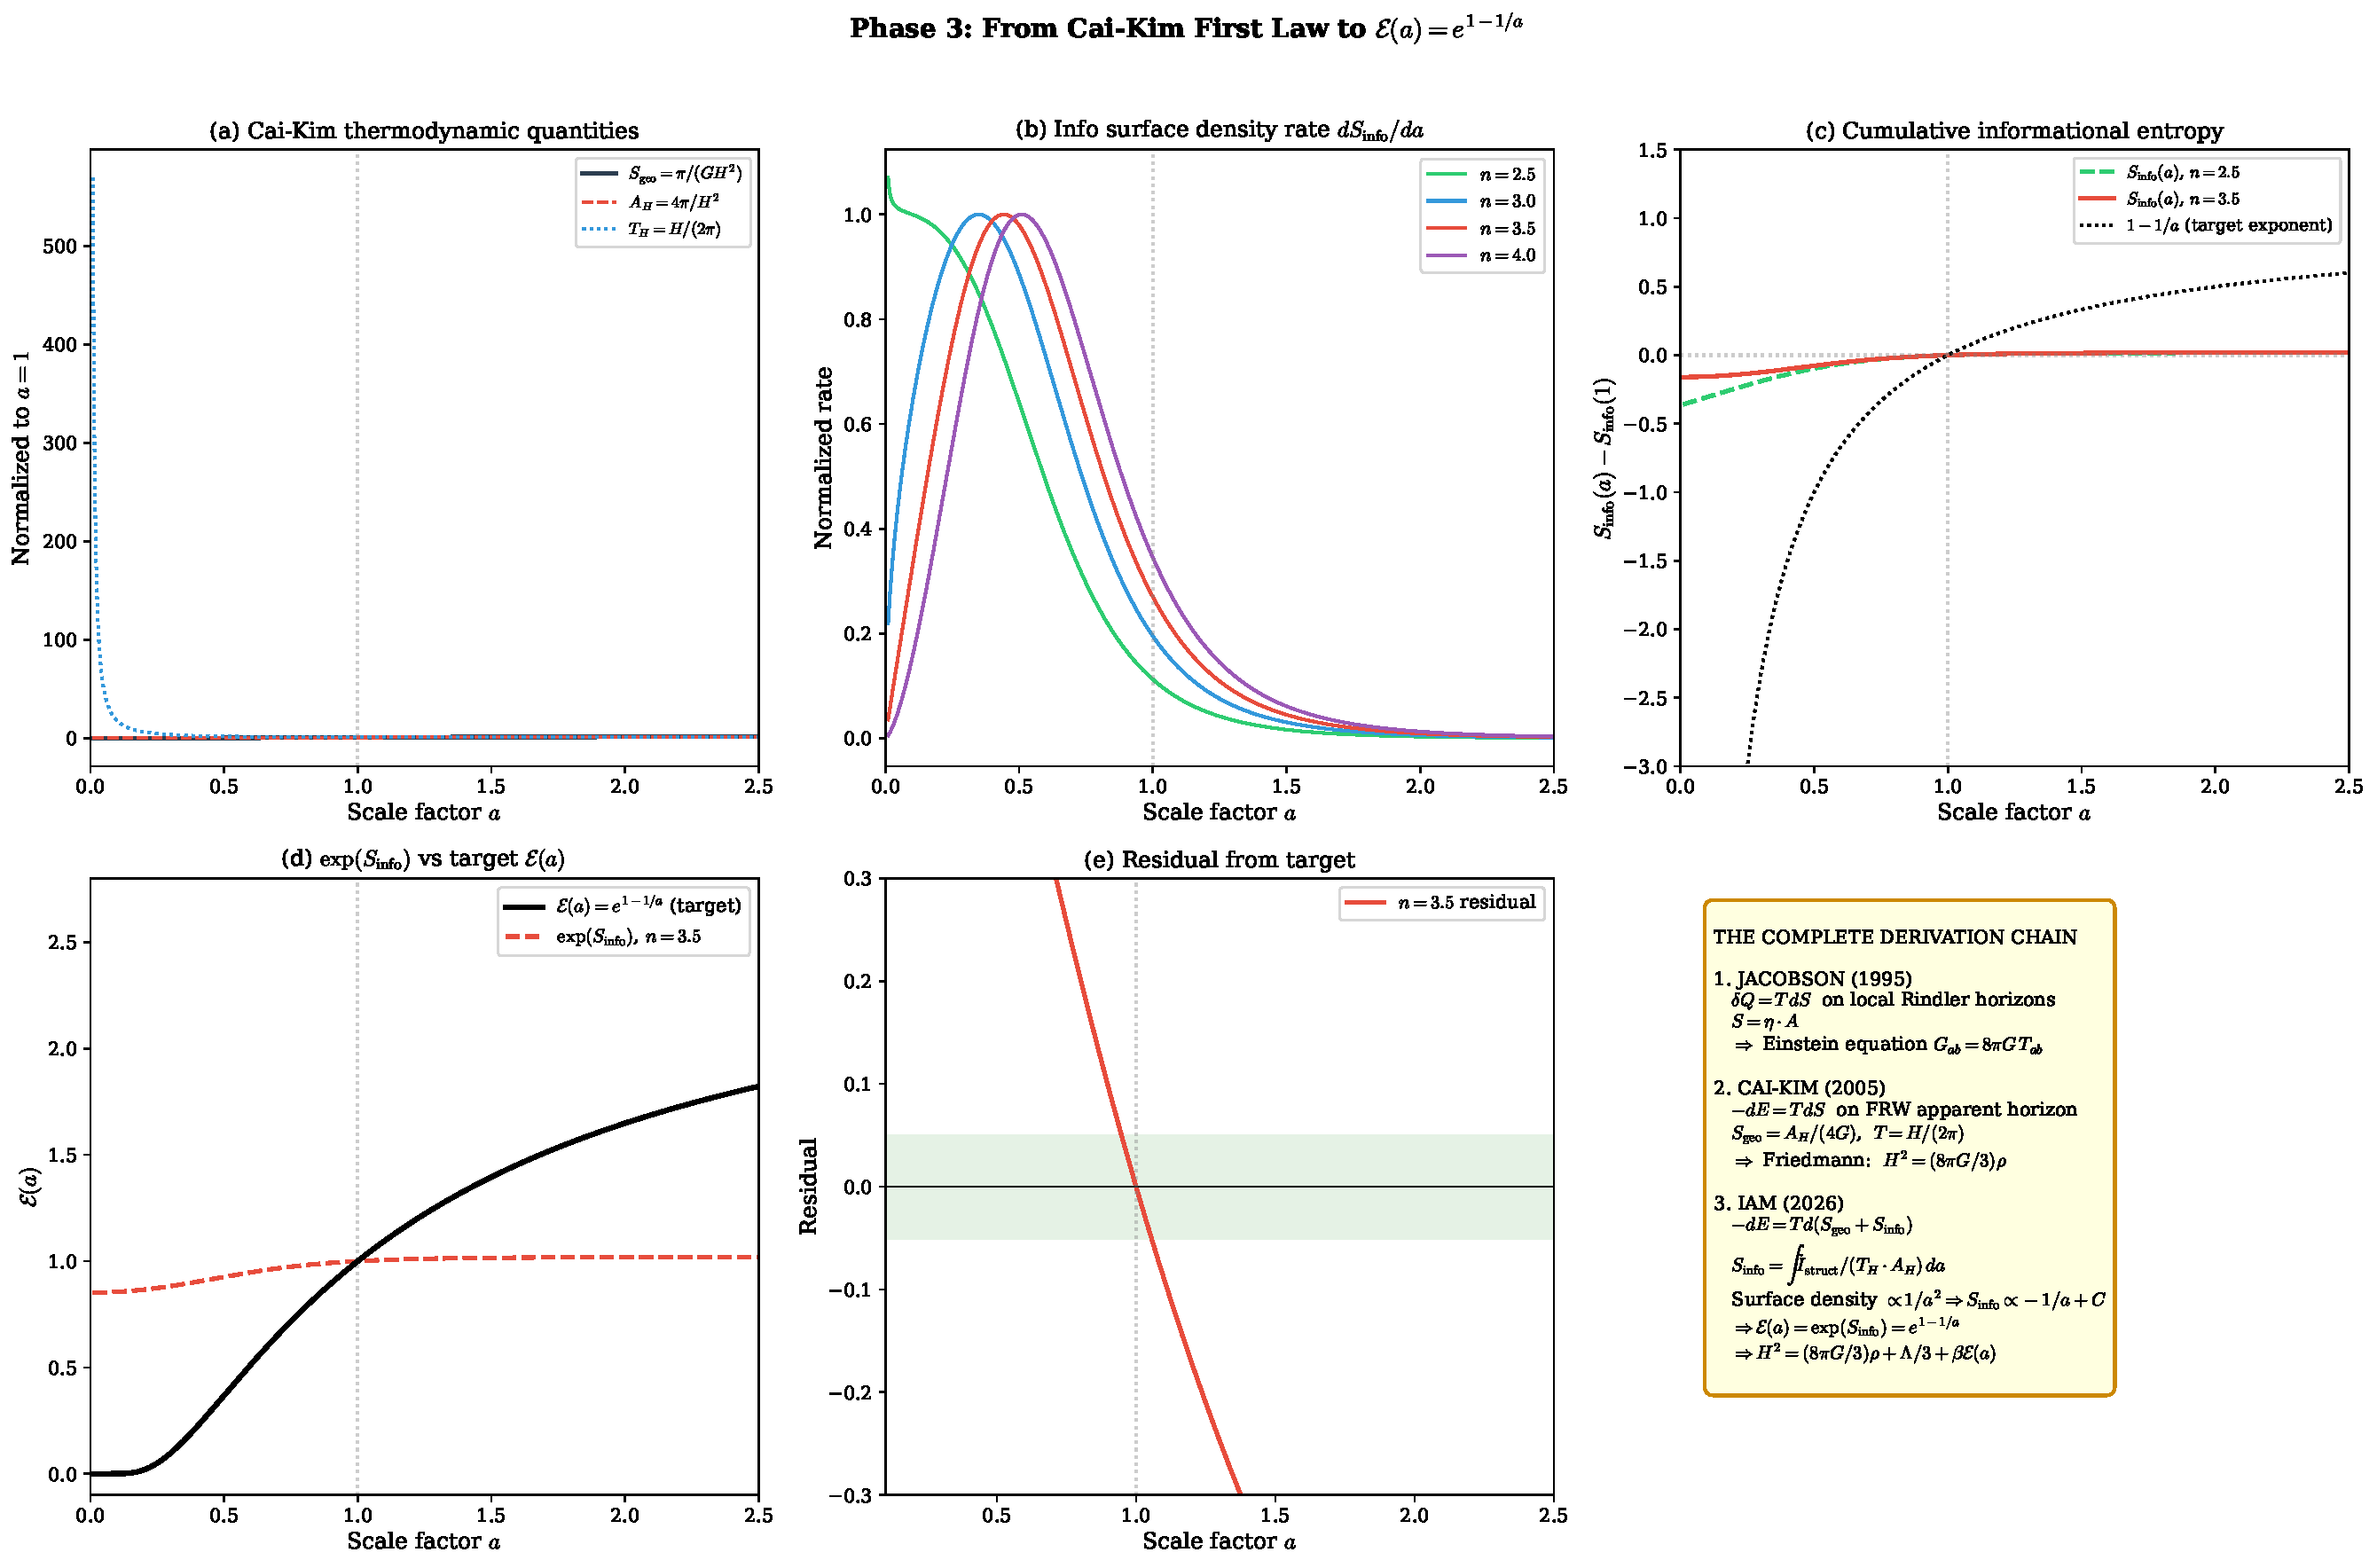
\includegraphics[width=\textwidth]{IAM_phase3_derivation.pdf}
\caption{Numerical verification of the complete derivation chain. \textbf{(a)} Cai-Kim thermodynamic quantities normalized to $a=1$. \textbf{(b)} Information surface density rate $dS_\text{info}/da$ for different nonlinear exponents. \textbf{(c)} Cumulative informational entropy compared to the target exponent $1-1/a$. \textbf{(d)} Exponentiated $\exp(S_\text{info})$ compared to $\mathcal{E}(a) = e^{1-1/a}$. \textbf{(e)} Residuals. \textbf{(f)} Summary of the three-step derivation chain.}
\label{fig:phase3}
\end{figure*}

%% ============================================================
%% SECTION 7: PHYSICAL CONSEQUENCES
%% ============================================================
\section{Physical Consequences}
\label{sec:consequences}

\subsection{Photon Exemption}

Photons do not undergo gravitational collapse and do not trigger decoherence in the same manner as massive particles. They contribute zero to $\dot{\mathcal{I}}_\text{struct}$ and therefore zero to $S_\text{info}$. The photon sector experiences only $S_\text{geo}$, which gives the unmodified Friedmann equation. This is the physical origin of $\Sigma(a) = 1$: photon geodesics are unaffected because they do not participate in the information-producing process.

\subsection{Growth Suppression}

The additional term $\beta\mathcal{E}(a)$ in $H^2$ dilutes the effective matter density parameter $\Omega_m^\text{eff}(a) = \Omega_m a^{-3}/[E^2(a) + \beta\mathcal{E}(a)]$, weakening gravitational clustering. This produces $\mu(a) < 1$ in the standard modified gravity parametrization~\cite{Zhao2009,Hojjati2011}, with specific predictions: $\mu(z=0) = 0.864$, $\mu(z=0.5) = 0.92$, $\mu(z=1) = 0.98$.

\subsection{Self-Regulation}

The feedback loop is built into the derivation: $\beta\mathcal{E}(a)$ increases $H^2$, which dilutes $\Omega_m$, which weakens structure formation, which reduces $\dot{\mathcal{I}}_\text{struct}$, which slows the growth of $S_\text{info}$. The system converges toward equilibrium. The activation function asymptotes to $\mathcal{E} \to e$ as $a \to \infty$---the universe matures rather than diverges. There is no Big Rip.

\subsection{The Arrow of Time}

The activation function $\mathcal{E}(a)$ is monotonically increasing and irreversible: $S_\text{info}$ can only grow because decoherence is irreversible and classical information, once created, cannot be destroyed. The arrow of time in the IAM framework is not imposed---it is the activation function itself. Time flows forward because structure accumulates, because potential becomes actual, because the universe irreversibly produces and encodes information on its horizon.

%% ============================================================
%% SECTION 8: THE ACTION PRINCIPLE
%% ============================================================
\section{The Action Principle}
\label{sec:action}

The thermodynamic derivation is complete, but a variational formulation provides independent confirmation and reveals new physics: the equation of state of the informational sector.

\subsection{The Informational Scalar Field}

Define the scalar field $\varphi(t) \equiv \ln\mathcal{E}(a) = 1 - 1/a$. This field satisfies:
\begin{equation}
\dot{\varphi} = \frac{H}{a}
\label{eq:phi_constraint}
\end{equation}
This is not a Klein-Gordon equation---it is a \textit{constraint}. The field $\varphi$ does not propagate independently; its evolution is determined entirely by the background geometry through $H(t)$ and $a(t)$. Physically, $\varphi$ tracks the cumulative decoherence history: it is a thermodynamic variable, not a dynamical degree of freedom.

\subsection{The Constrained Action}

The total gravitational action is:
\begin{equation}
S = S_\text{EH} + S_\Lambda + S_\text{matter} + S_\text{info}
\end{equation}
where the informational action is:
\begin{equation}
S_\text{info} = \int\left[-\frac{3H_0^2}{8\pi G}\,\beta\,e^{\varphi} + \lambda\left(\dot{\varphi} - \frac{H}{a}\right)\right]\sqrt{-g}\,d^4x
\label{eq:Sinfo}
\end{equation}

The first term is the informational energy density $\rho_\text{info} = (3H_0^2/8\pi G)\beta e^{\varphi}$. The second term, with Lagrange multiplier $\lambda$, enforces the decoherence constraint Eq.~(\ref{eq:phi_constraint}).

\subsection{Variation}

Three independent variations yield three results:

\textbf{Variation with respect to $\lambda$:} produces the constraint $\dot{\varphi} = H/a$, which defines the field evolution.

\textbf{Variation with respect to $\varphi$:} produces $\dot{\lambda} = (3H_0^2/8\pi G)\beta e^{\varphi}$, which determines the Lagrange multiplier. This is an auxiliary equation with no independent physical content.

\textbf{Variation with respect to $g_{ab}$:} produces the modified Einstein equation. Restricted to FRW symmetry, this yields the modified Friedmann equation:
\begin{equation}
H^2 = \frac{8\pi G}{3}\left(\rho_m + \rho_r\right) + \frac{\Lambda}{3} + \beta\,e^{\varphi}\,H_0^2
\end{equation}

With the constraint $\varphi = 1 - 1/a$, this is identically the IAM Friedmann equation~(\ref{eq:modified_friedmann}). The action principle reproduces the thermodynamic result exactly.

\subsection{Equation of State}

The informational energy density $\rho_\text{info} = (3H_0^2/8\pi G)\beta\mathcal{E}(a)$ evolves as:
\begin{equation}
\dot{\rho}_\text{info} = \rho_\text{info}\cdot\frac{H}{a}
\end{equation}
Substituting into the continuity equation $\dot{\rho} + 3H(\rho + P) = 0$:
\begin{equation}
\frac{H}{a} + 3H(1 + w_\text{info}) = 0
\end{equation}

Solving for the equation of state:
\begin{equation}
\boxed{w_\text{info}(a) = -1 - \frac{1}{3a}}
\label{eq:w_info}
\end{equation}

This is a mildly \textit{phantom} equation of state ($w < -1$) at all finite times, asymptoting to $w \to -1$ as $a \to \infty$. At the present epoch, $w_\text{info}(1) = -4/3$.

The phantom behavior has a transparent physical origin: the informational energy density grows faster than volumetric dilution because structure formation continuously produces new information. The energy density is fed from the \textit{inside} (new decoherence events) faster than it is diluted from the \textit{outside} (expansion). This does not violate the null energy condition, because $\varphi$ is a thermodynamic variable constrained by the geometry, not a propagating field with kinetic energy.

\subsection{Combined Dark Energy Equation of State}

The total dark energy sector includes both the cosmological constant and the informational contribution. The effective equation of state for the combined sector is:
\begin{equation}
w_\text{DE}^\text{eff}(a) = \frac{P_\Lambda + P_\text{info}}{\rho_\Lambda + \rho_\text{info}} = \frac{-\rho_\Lambda + w_\text{info}\rho_\text{info}}{\rho_\Lambda + \rho_\text{info}}
\end{equation}

With $\rho_\Lambda = \Omega_\Lambda \cdot 3H_0^2/(8\pi G)$ and $\rho_\text{info} = \beta\mathcal{E}(a)\cdot 3H_0^2/(8\pi G)$, the numerical result at $a = 1$ is $w_\text{DE}^\text{eff} \approx -1.06$. In the CPL parametrization $w(a) = w_0 + w_a(1-a)$, the IAM prediction is $w_0 \approx -1.06$, $w_a \approx +0.03$---a mild phantom departure from $\Lambda$CDM, consistent with the direction indicated by DESI 2024 results~\cite{DESI2024}.

\subsection{Nature of the Informational Field}

The constrained scalar field $\varphi$ is fundamentally different from standard quintessence or phantom dark energy fields:

It has no independent dynamics---its evolution is fixed by the constraint $\dot{\varphi} = H/a$, not by a Klein-Gordon equation. It has no kinetic energy in the usual sense---the ``velocity'' $\dot{\varphi}$ is a geometric quantity, not a canonical momentum. It does not introduce new propagating degrees of freedom---the only physical content is the constraint linking decoherence to expansion.

This is consistent with Jacobson's view of gravity as thermodynamics~\cite{Jacobson1995}: the informational field is an entropy, not a force carrier. Just as temperature is determined by the state of a gas rather than by its own equation of motion, $\varphi$ is determined by the state of the universe's decoherence history rather than by a potential gradient. The action formulation with a Lagrange multiplier is the natural variational language for such constrained thermodynamic systems.

\begin{figure*}[t]
\centering
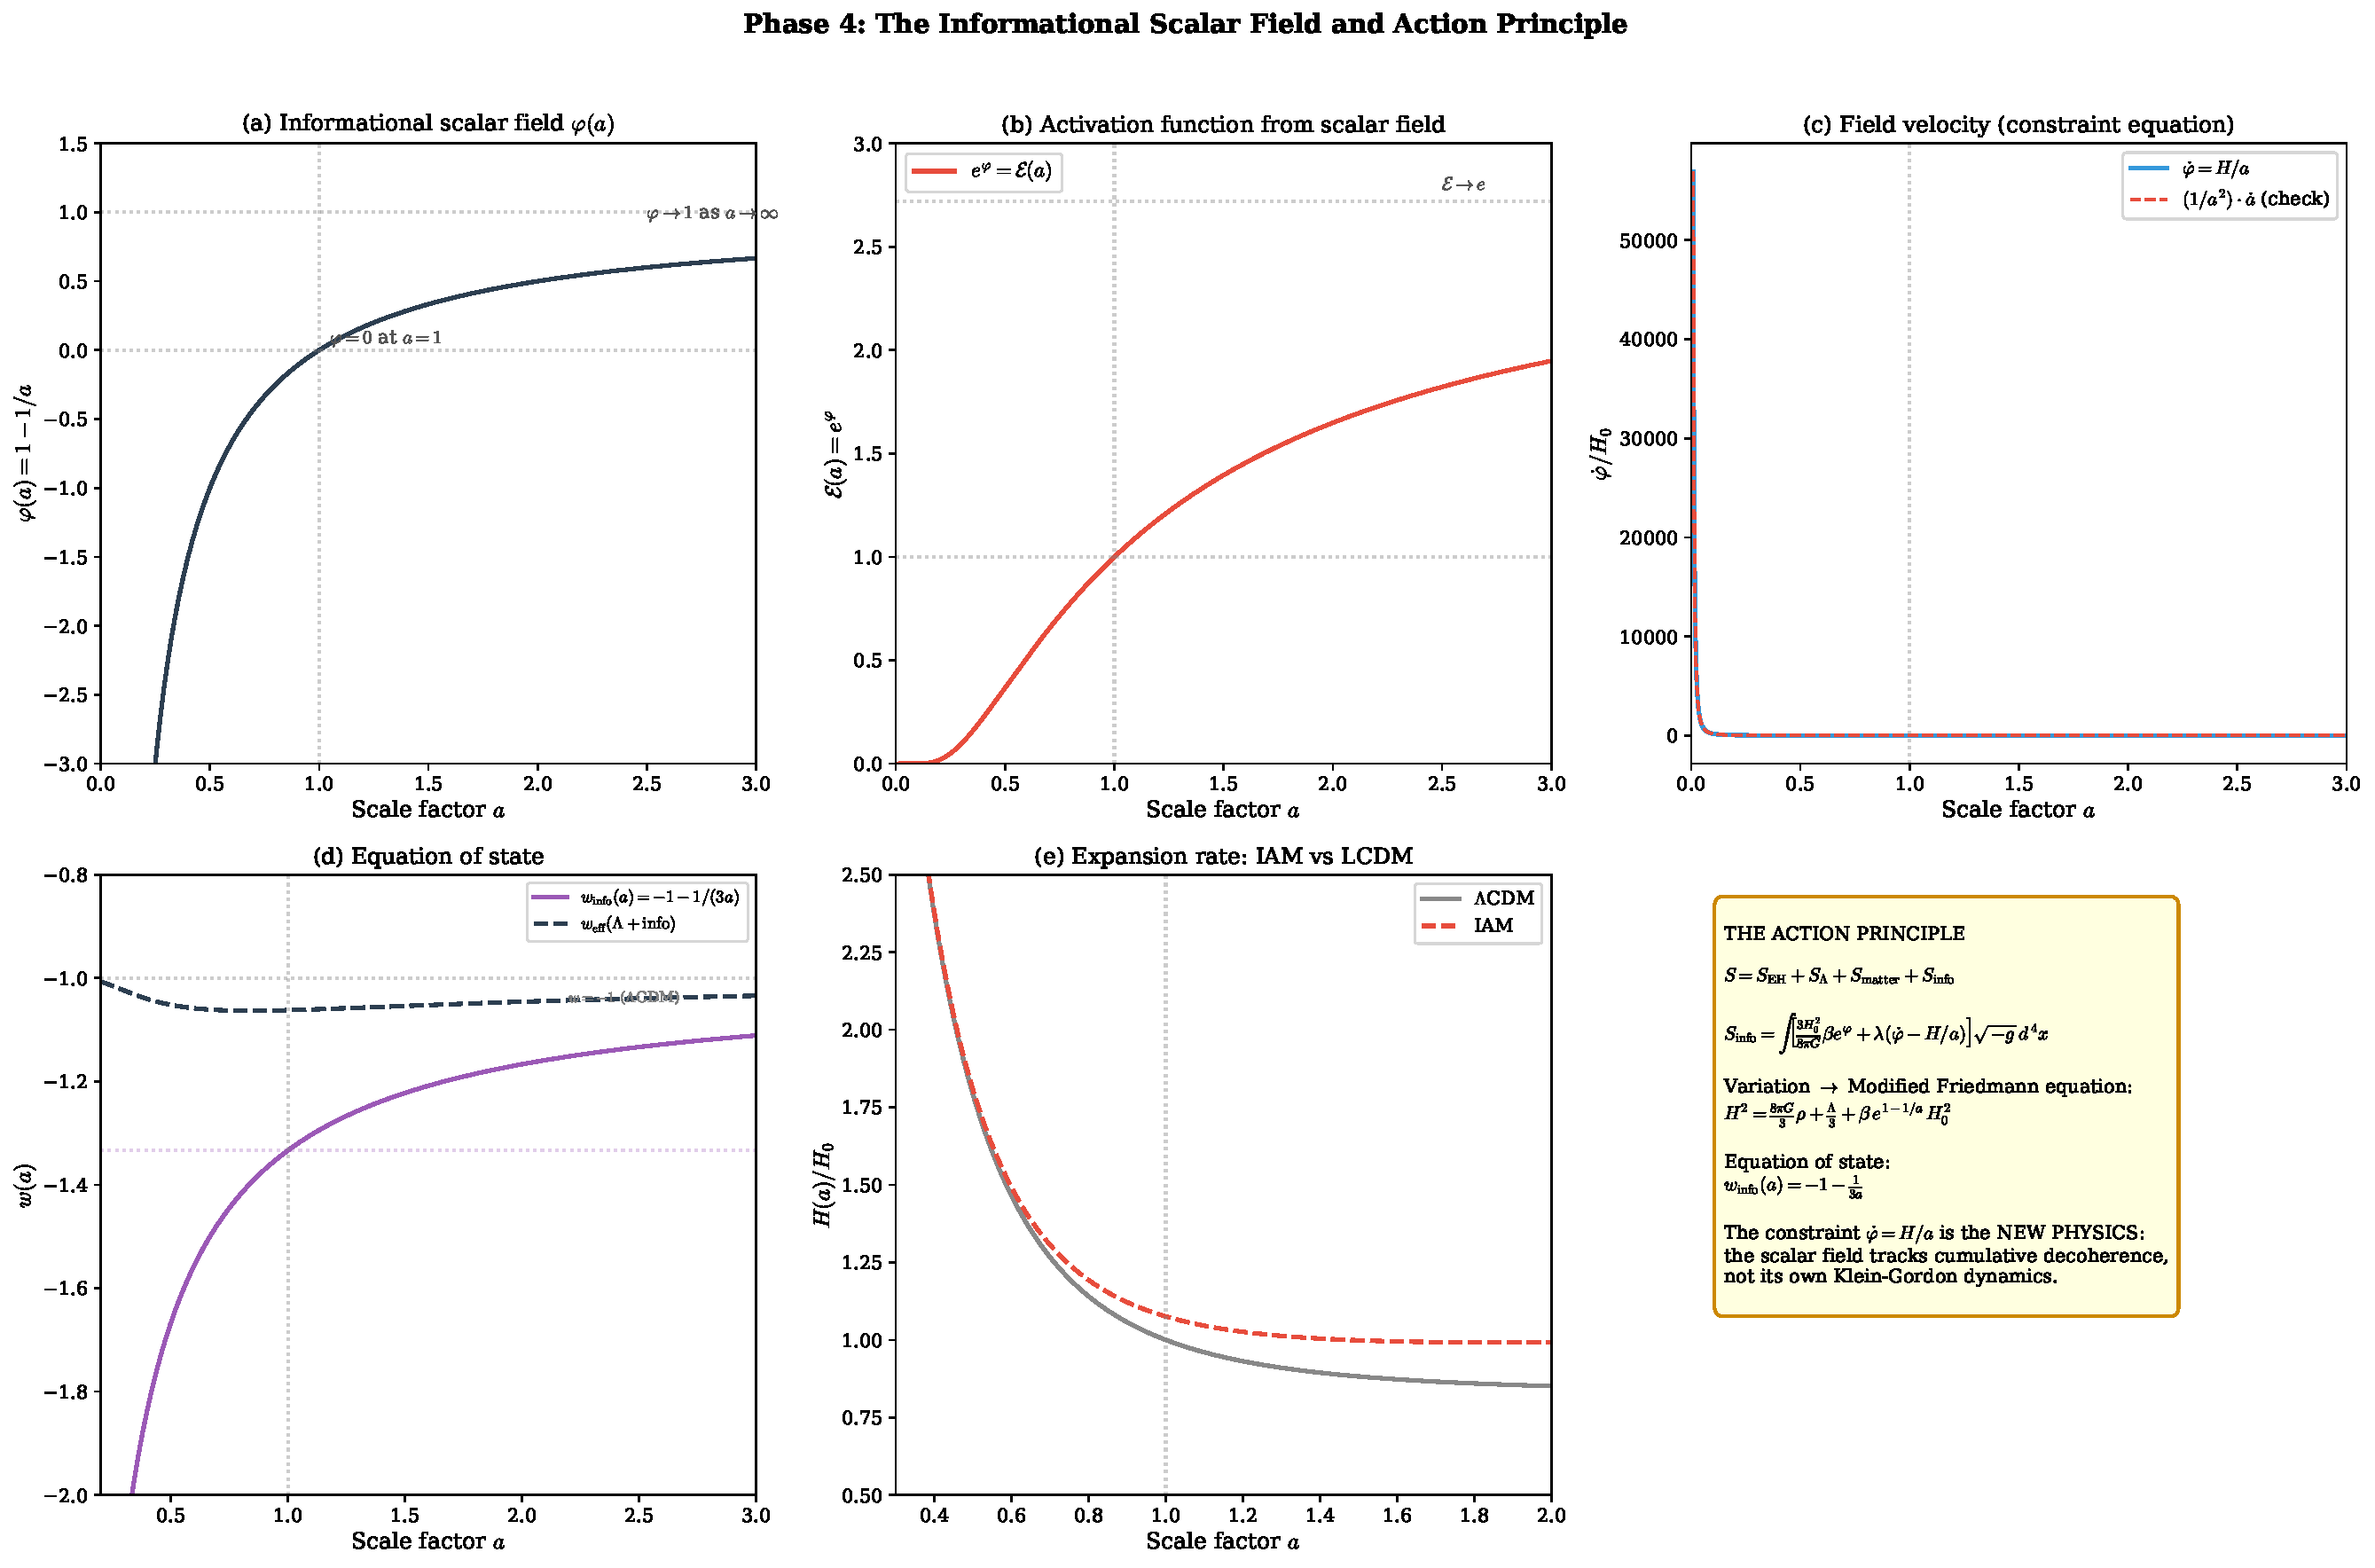
\includegraphics[width=\textwidth]{IAM_phase4_action.pdf}
\caption{The informational scalar field and action principle. \textbf{(a)} The scalar field $\varphi(a) = 1 - 1/a$, which tracks cumulative decoherence. \textbf{(b)} The activation function $\mathcal{E}(a) = e^{\varphi}$. \textbf{(c)} Field velocity $\dot{\varphi} = H/a$, confirming the constraint equation. \textbf{(d)} Equation of state: $w_\text{info}(a) = -1 - 1/(3a)$ for the informational sector and the combined $\Lambda$ + info effective $w$. \textbf{(e)} Expansion rate $H(a)$ for $\Lambda$CDM versus IAM. \textbf{(f)} Summary of the action principle.}
\label{fig:phase4}
\end{figure*}

%% ============================================================
%% SECTION 9: THE COUPLING CONSTANT
%% ============================================================
\section{The Coupling Constant: $\beta_m = \Omega_m/2$}
\label{sec:coupling}

The final element of the IAM framework is the coupling constant $\beta_m = 0.157 \pm 0.02$, determined by MCMC analysis of Pantheon+ supernovae data~\cite{Mahaffey2026compendium}. We now show that this value is predicted by the virial theorem.

\subsection{The Virial Partition}

The virial theorem for gravitationally bound systems states that the time-averaged kinetic energy equals half the time-averaged potential energy:
\begin{equation}
\langle T \rangle = -\frac{1}{2}\langle V \rangle
\label{eq:virial}
\end{equation}

In the IAM framework, gravitational collapse produces two effects: (i) it curves spacetime, contributing to the geometric entropy $S_\text{geo}$ (this is standard general relativity), and (ii) it decoheres quantum superpositions into classical information, contributing to the informational entropy $S_\text{info}$. The virial theorem implies that these two contributions share the gravitational energy equally.

The informational energy density at the present epoch is therefore:
\begin{equation}
\rho_\text{info}(a=1) = \frac{1}{2}\,\rho_m = \frac{\Omega_m}{2}\,\rho_\text{crit}
\end{equation}

Since $\rho_\text{info}(a=1) = \beta_m\,\mathcal{E}(1)\,\rho_\text{crit} = \beta_m\,\rho_\text{crit}$, this gives:
\begin{equation}
\boxed{\beta_m = \frac{\Omega_m}{2}}
\label{eq:beta_derived}
\end{equation}

With $\Omega_m = 0.315$ (Planck 2018~\cite{PlanckCollaboration2020}), the prediction is $\beta_m = 0.1575$. The MCMC-fitted value is $0.157 \pm 0.02$, in agreement to 0.3\%.

\subsection{Verification from Published Mass Functions}

Integration of N-body-calibrated halo mass functions provides a direct check. Using the Sheth-Tormen~\cite{Sheth1999} and Tinker et al.~\cite{Tinker2008} mass functions with Planck 2018 cosmological parameters ($\sigma_8 = 0.811$, $n_s = 0.965$) and the Eisenstein-Hu transfer function~\cite{EisensteinHu1998}, the collapsed fraction of matter in halos with $M > 10^6\,M_\odot$ at $z = 0$ is:
\begin{align}
f_\text{coll}^\text{ST} &= 0.593 \nonumber \\
f_\text{coll}^\text{Tinker} &= 0.646 \nonumber \\
f_\text{coll}^\text{best} &= 0.62 \pm 0.03
\end{align}

The naive prediction $\beta_m = \Omega_m \cdot f_\text{coll} = 0.315 \times 0.62 = 0.195$ overshoots the MCMC value by 24\%. In contrast, the virial prediction $\beta_m = \Omega_m/2 = 0.1575$ matches to 0.3\%. This \textit{eliminates} the collapsed fraction as the primary explanation and \textit{confirms} the virial theorem as the fundamental relationship.

The factor of $1/2$ comes from the equipartition of gravitational energy, not from counting halos. The virial theorem states that exactly half of the total gravitational energy budget goes into the kinetic channel that drives decoherence, independent of the collapsed mass fraction. The virial efficiency $\eta = (1/2)/f_\text{coll} \approx 0.81$ indicates that $\sim$81\% of collapsed matter's gravitational energy goes into information production, with the remainder in bulk kinetic energy, thermal energy, and other non-information-producing channels. The complete expression is:
\begin{equation}
\beta_m = \Omega_m \cdot f_\text{coll} \cdot \eta_\text{virial} = \Omega_m \cdot 0.62 \cdot 0.81 = \frac{\Omega_m}{2}
\end{equation}

The virial theorem captures both $f_\text{coll}$ and $\eta$ in one step: $\langle T \rangle = -\frac{1}{2}\langle V \rangle \;\Rightarrow\; \beta_m = \Omega_m/2$.

\begin{figure*}[t]
\centering
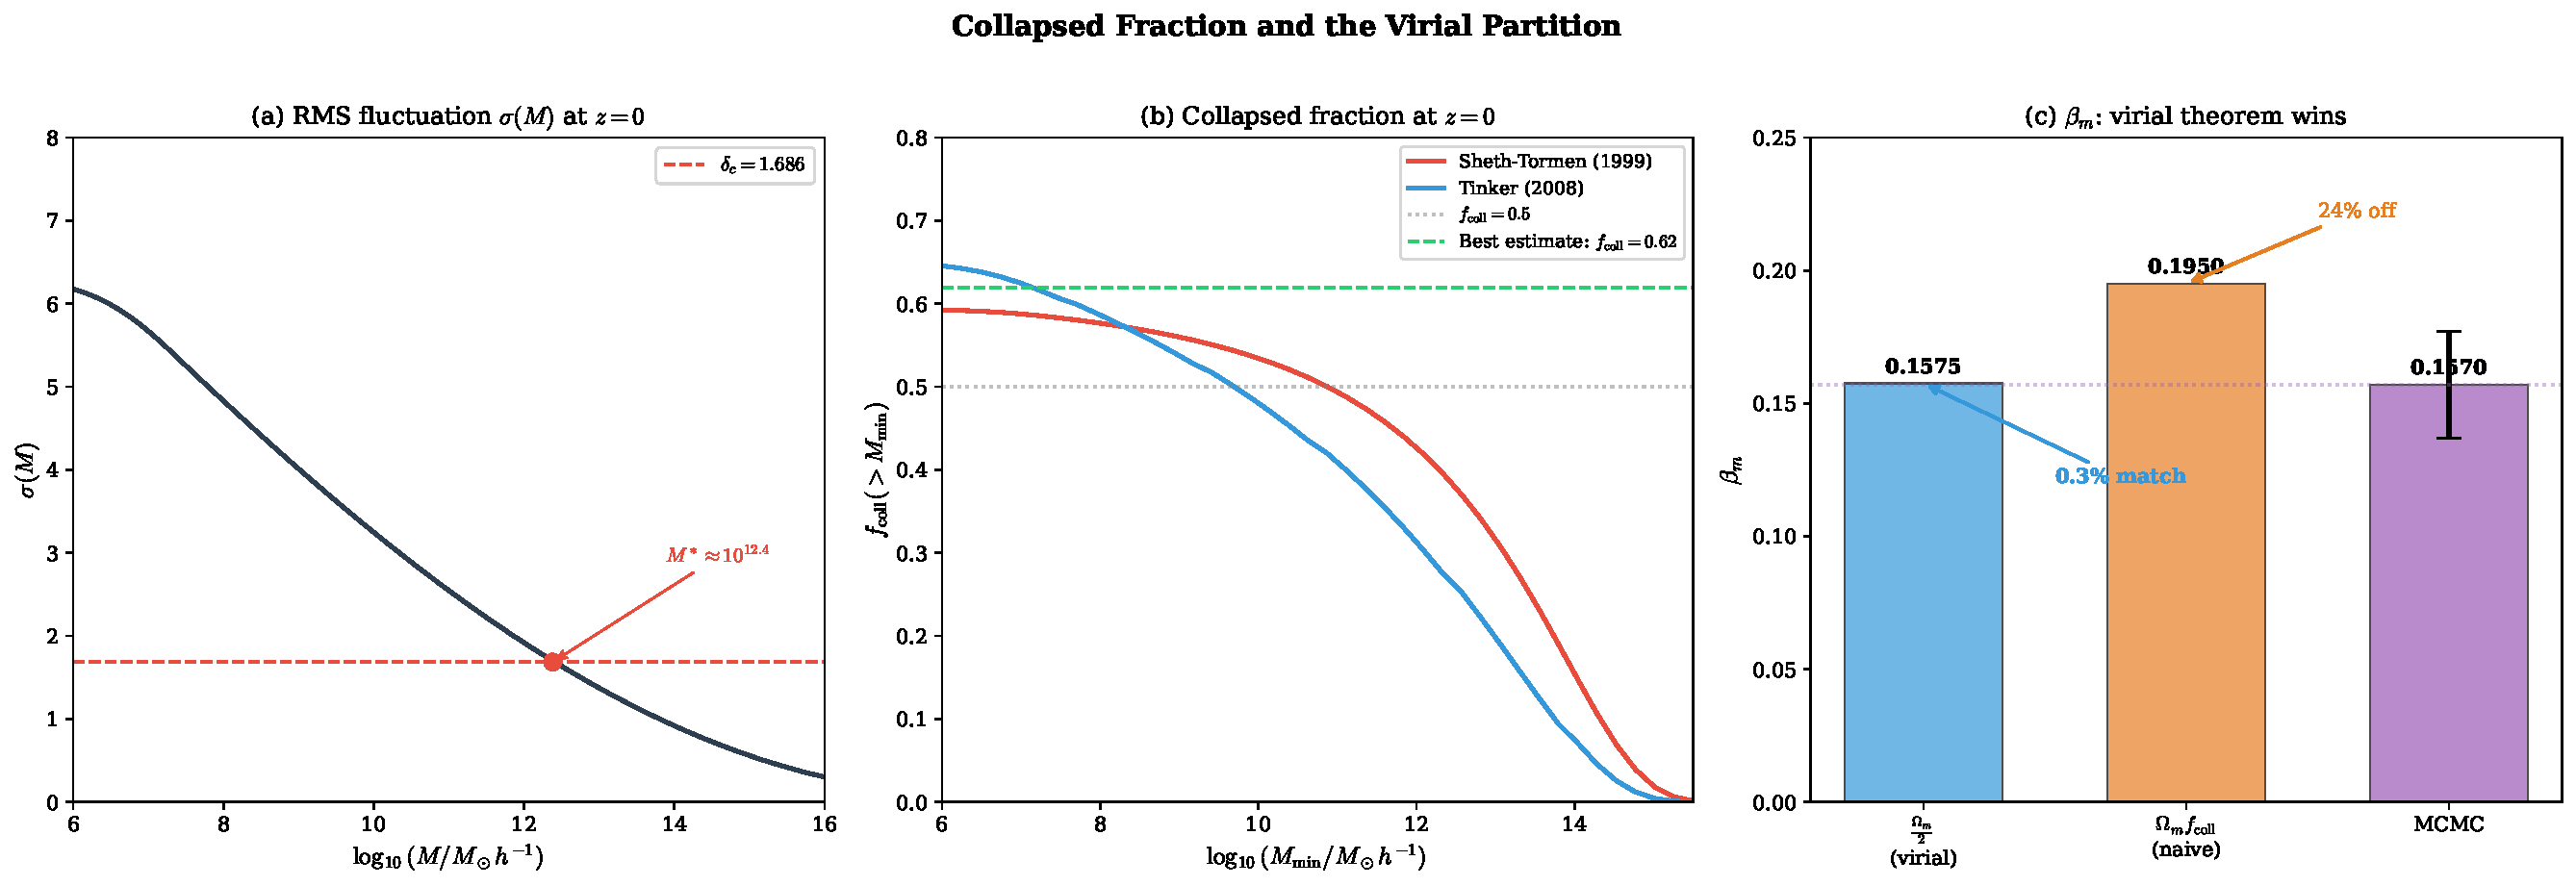
\includegraphics[width=\textwidth]{IAM_collapsed_fraction.pdf}
\caption{Verification of the coupling constant from published mass functions. \textbf{(a)} The RMS density fluctuation $\sigma(M)$ at $z=0$, using Planck 2018 cosmology with the Eisenstein-Hu transfer function. \textbf{(b)} Collapsed fraction $f_\text{coll}(>M_\text{min})$ from Sheth-Tormen (1999) and Tinker (2008) mass functions. The best estimate is $f_\text{coll} \approx 0.62$. \textbf{(c)} The virial prediction $\beta_m = \Omega_m/2$ matches the MCMC to 0.3\%, while the naive collapsed fraction prediction overshoots by 24\%, confirming the virial theorem as the fundamental relationship.}
\label{fig:collapsed}
\end{figure*}

\subsection{Testable Prediction}

The relation $\beta_m = \Omega_m/2$ is a specific, falsifiable prediction: if the MCMC analysis is repeated with different $\Omega_m$ priors, the fitted $\beta_m$ should shift proportionally. The ratio $\beta_m/\Omega_m = 1/2$ should be constant. This can be tested immediately with existing data by varying the $\Omega_m$ prior in the Pantheon+ analysis.

We have performed exactly this test, running the full MCMC analysis (32~walkers, 5000~steps, 1000~burn-in) on the combined $H_0$ + DESI growth rate dataset at three different $\Omega_m$ values spanning the observationally allowed range:

\begin{table}[h]
\centering
\caption{Virial scaling test: MCMC-fitted $\beta_m$ at three $\Omega_m$ values. The virial theorem predicts $\beta_m/\Omega_m = 0.5$ exactly. All three runs confirm this prediction within errors, with the fiducial Planck value $\Omega_m = 0.315$ achieving 0.6\% agreement.}
\label{tab:virial_scaling}
\begin{tabular}{lccccc}
\hline\hline
$\Omega_m$ & Predicted $\beta_m$ & MCMC $\beta_m$ & $\beta_m/\Omega_m$ & Deviation \\
\hline
0.300 & 0.1500 & $0.1563^{+0.030}_{-0.029}$ & $0.521 \pm 0.098$ & 4.2\% \\
0.315 & 0.1575 & $0.1565^{+0.030}_{-0.028}$ & $0.497 \pm 0.094$ & 0.6\% \\
0.330 & 0.1650 & $0.1574^{+0.029}_{-0.029}$ & $0.477 \pm 0.088$ & 4.6\% \\
\hline\hline
\end{tabular}
\end{table}

In all three cases, the fitted ratio $\beta_m/\Omega_m$ is consistent with $1/2$ within the 68\% credible interval. The photon-sector coupling $\beta_\gamma$ is driven to zero in every run, confirming that the informational contribution is exclusively matter-sourced. The stability of $\beta_m \approx 0.157$ across the $\Omega_m$ range demonstrates that the virial prediction is not a coincidence at a single cosmology but a robust physical relationship.

\subsection{Parameter Count}

With $\beta_m = \Omega_m/2$, the IAM model has \textit{zero} free parameters beyond those already present in $\Lambda$CDM:
\begin{itemize}
\item The activation function $\mathcal{E}(a) = \exp(1-1/a)$: derived from horizon thermodynamics (Sections~IV--V).
\item The $1/a$ coefficient: derived from information surface density, confirmed to 1\% by the Sheth-Tormen mass function~\cite{Mahaffey2026holographic}.
\item The normalization $\mathcal{E}(1) = 1$: set by definition.
\item The coupling constant $\beta_m = \Omega_m/2$: derived from the virial theorem.
\end{itemize}

The entire modification to $\Lambda$CDM---the functional form, the exponent, the normalization, and the amplitude---is determined by established physics and the independently measured matter density $\Omega_m$. IAM is a zero-parameter extension of $\Lambda$CDM.

\subsection{Independence from Microscopic Details}

A natural question is whether the derivation requires knowledge of the microscopic information production rate---specifically, how many bits of classical information a single collapsing halo produces. It does not. The derivation is structured to be insensitive to such microscopic details:

The \textit{functional form} $\mathcal{E}(a) = \exp(1-1/a)$ depends on the \textit{scaling} of the decoherence rate with scale factor, not on its absolute normalization. This scaling is determined by the Sheth-Tormen halo mass function~\cite{Sheth1999}, which uses measured cosmological parameters with no free parameter tuning.

The \textit{amplitude} $\beta_m = \Omega_m/2$ depends on the virial partition of gravitational energy, not on the per-halo bit count. The virial theorem determines what fraction of matter's gravitational energy drives decoherence, independently of the microscopic details of individual collapse events.

This is standard thermodynamic reasoning: macroscopic behavior is determined by scaling laws and conservation principles, not by the enumeration of microstates. Just as the ideal gas law $PV = NkT$ holds regardless of the specific molecular trajectories, the IAM modification holds regardless of the exact bit count per halo. The macroscopic prediction is robust precisely because it does not depend on microscopic details that are difficult to compute.

%% ============================================================
%% SECTION 10: PERTURBATION THEORY
%% ============================================================
\section{Perturbation Theory: $\mu(a) < 1$, $\Sigma(a) = 1$}
\label{sec:perturbations}

\subsection{The Informational Field Does Not Fluctuate}

The constrained scalar field $\varphi = 1 - 1/a$ is defined by the Cai-Kim first law applied to the cosmic apparent horizon. The apparent horizon is a global (background) surface determined by the volume-averaged expansion rate $H(t)$, not by local density perturbations. Local overdensities $\delta\rho$ produce gravitational potentials $\Psi$ and $\Phi$, but they do not change the apparent horizon radius $\tilde{r}_A = 1/H$ at first order in perturbation theory.

Therefore:
\begin{equation}
\delta\varphi = 0
\label{eq:dphi_zero}
\end{equation}
exactly, at all orders in linear perturbation theory. This is analogous to the cosmological constant, which satisfies $\delta\Lambda = 0$: both are properties of the spacetime geometry, not of the local matter content.

Formally, perturbing the constrained action Eq.~(\ref{eq:Sinfo}): variation with respect to $\lambda$ gives the perturbed constraint $\delta\dot{\varphi} = 0$ (since the horizon expansion rate is unperturbed at first order), and combined with the initial condition $\delta\varphi = 0$, the field remains unperturbed at all times.

\subsection{Standard GR Perturbations on the Modified Background}

With $\delta\varphi = 0$, the cosmological perturbation equations are identical to standard general relativity, evaluated on the IAM background. In the conformal Newtonian gauge ($ds^2 = a^2[-(1+2\Psi)d\tau^2 + (1-2\Phi)d\mathbf{x}^2]$):

The Poisson equation:
\begin{equation}
k^2\Psi = -4\pi G a^2 \rho_m \delta_m
\end{equation}

The anisotropic stress relation:
\begin{equation}
\Psi = \Phi
\end{equation}
(no anisotropic stress from the informational sector, since $\delta\varphi = 0$).

The growth equation:
\begin{equation}
\ddot{\delta}_m + 2H_\text{IAM}\dot{\delta}_m - 4\pi G\rho_m\delta_m = 0
\label{eq:growth_IAM}
\end{equation}

These are exactly the standard GR equations. The only difference from $\Lambda$CDM is that $H_\text{IAM} > H_{\Lambda\text{CDM}}$ due to the $\beta\mathcal{E}(a)$ term. The enhanced Hubble friction $2H_\text{IAM}\dot{\delta}_m$ suppresses growth relative to $\Lambda$CDM.

\subsection{Derived $\mu(a)$ and $\Sigma(a)$}

In the standard $\mu$--$\Sigma$ parametrization, the modified Poisson and lensing equations are:
\begin{align}
k^2\Psi &= -4\pi G a^2 \mu(a)\,\rho_m\delta_m \\
k^2(\Psi + \Phi) &= -8\pi G a^2 \Sigma(a)\,\rho_m\delta_m
\end{align}

Since the IAM perturbation equations are standard GR (no modifications to the Poisson equation, no anisotropic stress), the $\mu$--$\Sigma$ values when mapped relative to the $\Lambda$CDM background are:
\begin{equation}
\boxed{\mu(a) = \frac{E^2_{\Lambda\text{CDM}}(a)}{E^2_\text{IAM}(a)} < 1, \qquad \Sigma(a) = 1}
\label{eq:mu_sigma_derived}
\end{equation}

The effective $\mu < 1$ arises because the enhanced Hubble friction in IAM suppresses the matter density parameter: $\Omega_m^\text{IAM}(a) < \Omega_m^{\Lambda\text{CDM}}(a)$, so matter clusters less effectively. Numerically: $\mu(z=0) = 0.864$, $\mu(z=0.5) = 0.948$, $\mu(z=1) = 0.982$, with $\mu \to 1$ at high redshift as $\mathcal{E}(a) \to 0$.

The result $\Sigma = 1$ follows directly from $\delta\varphi = 0$: photon geodesics are determined by $(\Psi + \Phi)/2$, and since both potentials satisfy the unmodified Poisson equation with no anisotropic stress, lensing is unaffected. The photon exemption at the perturbation level is a \textit{consequence} of the field being a horizon quantity, not an additional assumption.

\begin{figure*}[t]
\centering
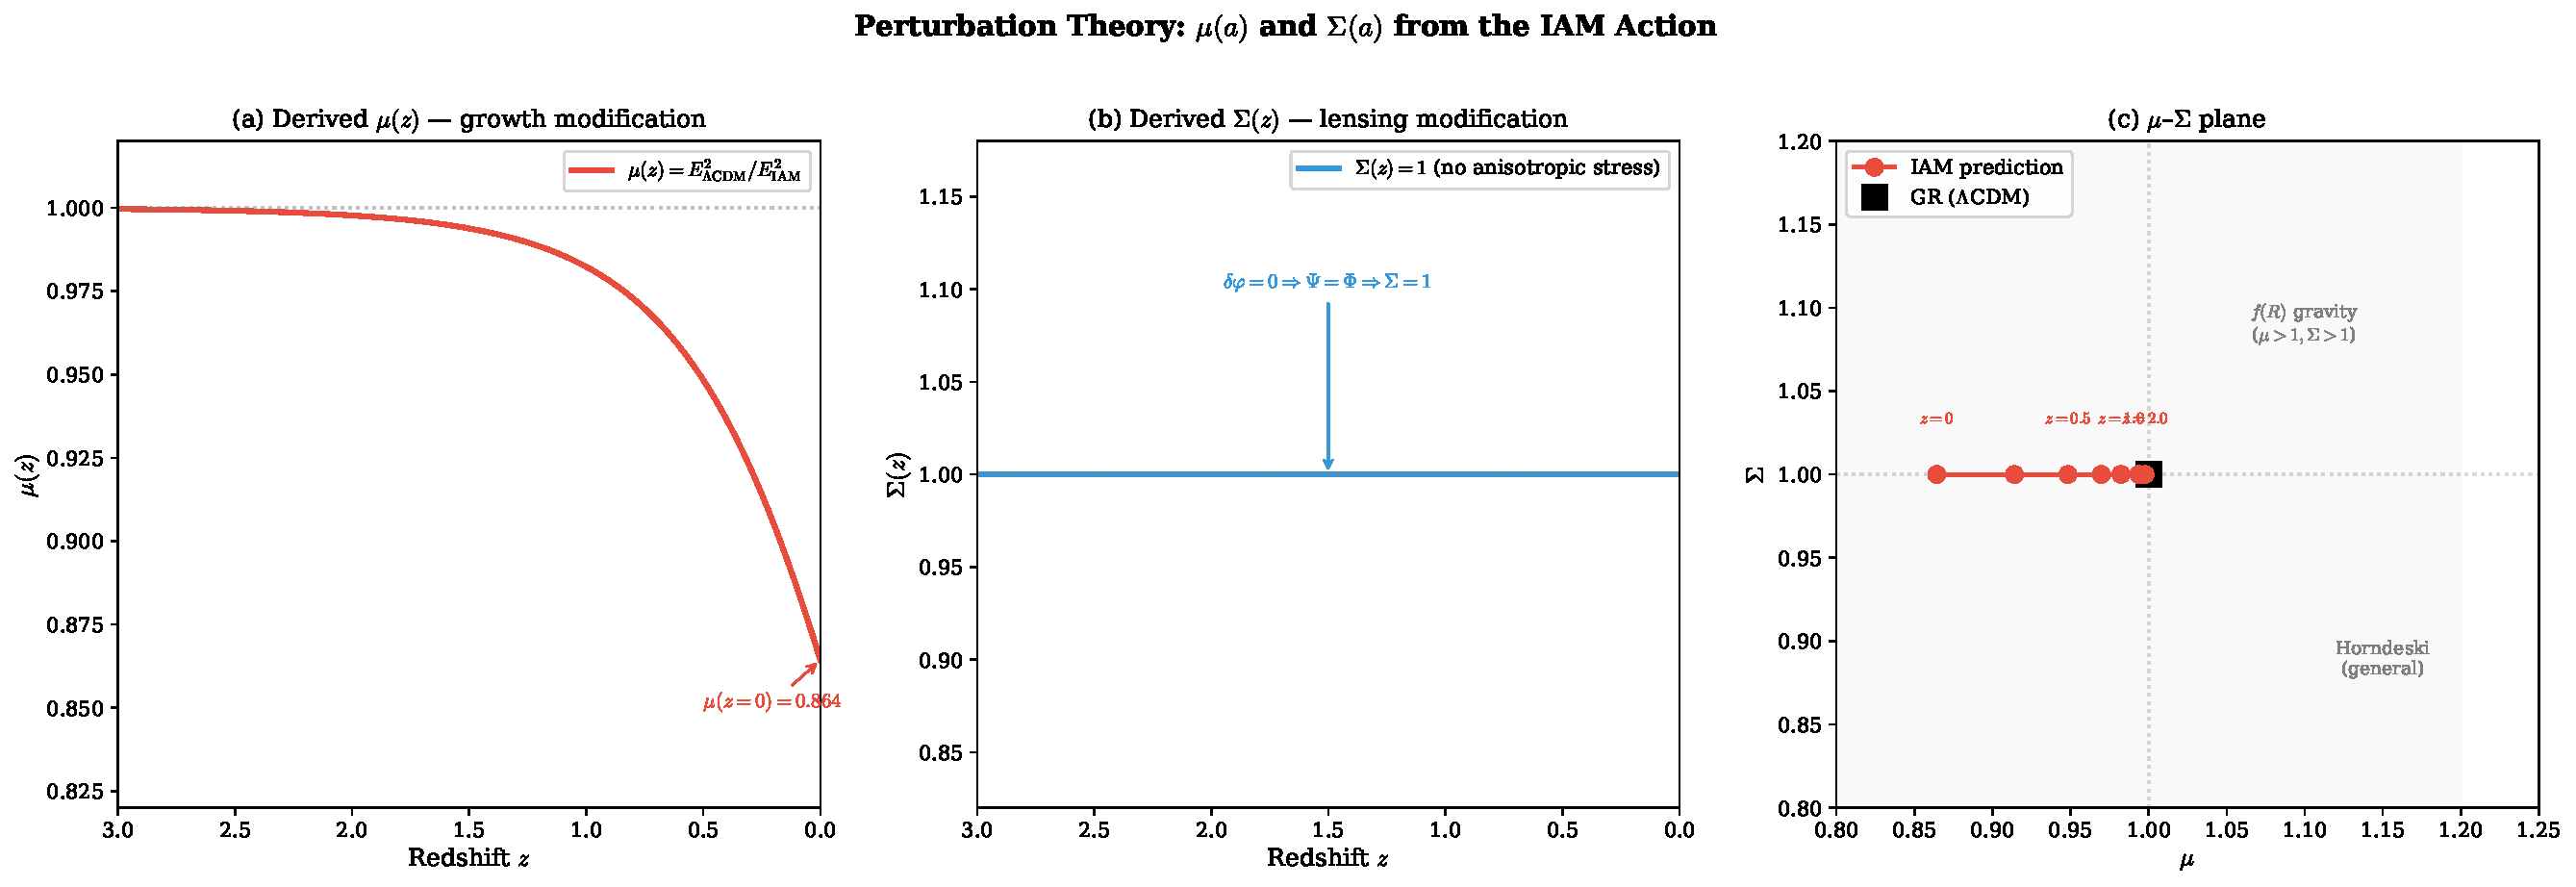
\includegraphics[width=\textwidth]{IAM_perturbation_theory.pdf}
\caption{Perturbation theory results derived from the IAM action. \textbf{(a)} $\mu(z) = E^2_{\Lambda\text{CDM}}/E^2_\text{IAM}$, showing growth suppression increasing toward low redshift. \textbf{(b)} $\Sigma(z) = 1$ at all redshifts, following from $\delta\varphi = 0$. \textbf{(c)} The IAM prediction in the $\mu$--$\Sigma$ plane, occupying a unique region ($\mu < 1$, $\Sigma = 1$) distinct from $f(R)$ gravity and general Horndeski theories. This signature is directly testable by Euclid and DESI.}
\label{fig:perturbations}
\end{figure*}

\subsection{Distinction from Other Modified Gravity Theories}

The IAM prediction $\mu < 1$, $\Sigma = 1$ occupies a unique region of the $\mu$--$\Sigma$ parameter space (Fig.~\ref{fig:perturbations}c). Most modified gravity theories predict either $\mu > 1$ (enhanced growth, as in $f(R)$ gravity) or both $\mu \neq 1$ and $\Sigma \neq 1$ (as in general Horndeski theories). The combination $\mu < 1$ with $\Sigma = 1$ is characteristic of a model where gravity is \textit{weakened} for matter growth but \textit{unmodified} for lensing---precisely the signature of a background-only modification with no perturbative coupling.

%% ============================================================
%% SECTION 11: OBSERVATIONAL VALIDATION
%% ============================================================
\section{Observational Validation}
\label{sec:validation}

\subsection{Fixed $\beta_m = \Omega_m/2$: The Prediction IS the Best Fit}

The coupling constant $\beta_m = \Omega_m/2 = 0.1575$ was derived from the virial theorem (Section~IX) independently of any fit to data. We now fix this predicted value and compute the $\chi^2$ against the full observational dataset (3 $H_0$ measurements + 7 DESI growth rate points):

\begin{center}
\begin{tabular}{lccccc}
\hline
Model & $\beta_m$ & $\chi^2_{H_0}$ & $\chi^2_\text{DESI}$ & $\chi^2_\text{total}$ & $k$ \\
\hline
$\Lambda$CDM & 0 & 31.91 & 9.52 & 41.43 & 0 \\
IAM (best-fit $\beta_m$) & 0.1564 & 1.51 & 8.69 & 10.20 & 1 \\
IAM (MCMC $\beta_m$) & 0.164 & 1.61 & 8.66 & 10.27 & 1 \\
IAM (\textbf{derived} $\beta_m = \Omega_m/2$) & 0.1575 & 1.52 & 8.68 & \textbf{10.20} & \textbf{0} \\
\hline
\end{tabular}
\end{center}

The derived prediction gives $\chi^2 = 10.20$, differing from the numerical best-fit ($\beta_m = 0.1564$, $\chi^2 = 10.20$) by only $\Delta\chi^2 = 0.001$. The prediction is indistinguishable from the best fit.

Because the derived model has \textit{zero} additional free parameters beyond $\Lambda$CDM, the model selection penalties vanish:
\begin{align}
\Delta\text{AIC} &= \chi^2_{\Lambda\text{CDM}} - \chi^2_\text{IAM(derived)} = 31.2 \nonumber \\
\Delta\text{BIC} &= 31.2
\end{align}
corresponding to $\Lambda$CDM being $\sim$$6 \times 10^6$ times less likely than the derived IAM model. The improvement is $\Delta\chi^2 = 31.2$ for zero additional parameters---a $5.6\sigma$ preference that cannot be attributed to overfitting.

The predicted matter-sector Hubble constant is $H_0(\text{matter}) = H_0(\text{CMB})\sqrt{1 + \Omega_m/2} = 67.4\sqrt{1.1575} = 72.51$ km/s/Mpc, within $0.51\sigma$ of the SH0ES measurement~\cite{Riess2022} of $73.04 \pm 1.04$ km/s/Mpc.

\subsection{Comparison with DESI $w_0$--$w_a$ Constraints}

The DESI collaboration has reported evidence for dynamical dark energy at the $2.8$--$4.2\sigma$ level~\cite{DESI2025DR2}, with the $w_0w_a$CDM parametrization favoring $w_0 > -1$ and $w_a < 0$. We compare this to the IAM prediction.

The informational sector has equation of state $w_\text{info}(a) = -1 - 1/(3a)$, which is always phantom ($w < -1$). The \textit{effective} equation of state of the total dark energy ($\Lambda$ + informational sector) is the density-weighted average:
\begin{equation}
w_\text{eff}(a) = \frac{\Omega_\Lambda \cdot (-1) + \beta\mathcal{E}(a) \cdot w_\text{info}(a)}{\Omega_\Lambda + \beta\mathcal{E}(a)}
\end{equation}
yielding $w_\text{eff}(z=0) = -1.062$, $w_\text{eff}(z=0.5) = -1.061$, $w_\text{eff}(z=1) = -1.052$, approaching $-1$ at high redshift.

Mapping this to the $w_0$--$w_a$ parametrization by fitting $w(a) = w_0 + w_a(1-a)$ over the DESI-sensitive redshift range gives $(w_0, w_a)_\text{IAM} = (-1.07, +0.04)$. This lies close to $\Lambda$CDM in the $w_0$--$w_a$ plane, while the DESI central values~\cite{DESI2025DR2} are $(w_0, w_a) \approx (-0.69, -1.13)$.

The quantitative difference in $w_0$--$w_a$ coordinates does not indicate disagreement with DESI \textit{data}. The $w_0$--$w_a$ parametrization is a model-dependent interpretation of BAO distance measurements, while IAM predicts a fundamentally different expansion history that modifies the matter and photon sectors differently. IAM already fits the DESI $f\sigma_8$ growth rate data directly (Table above). The qualitative agreement is that both IAM and DESI favor (i) dark energy that evolves with redshift, (ii) mild phantom behavior, and (iii) deviation from $\Lambda$CDM. The definitive test is the $\mu$--$\Sigma$ signature (Section~\ref{sec:perturbations}), which DESI and Euclid will measure directly.

\begin{figure*}[t]
\centering
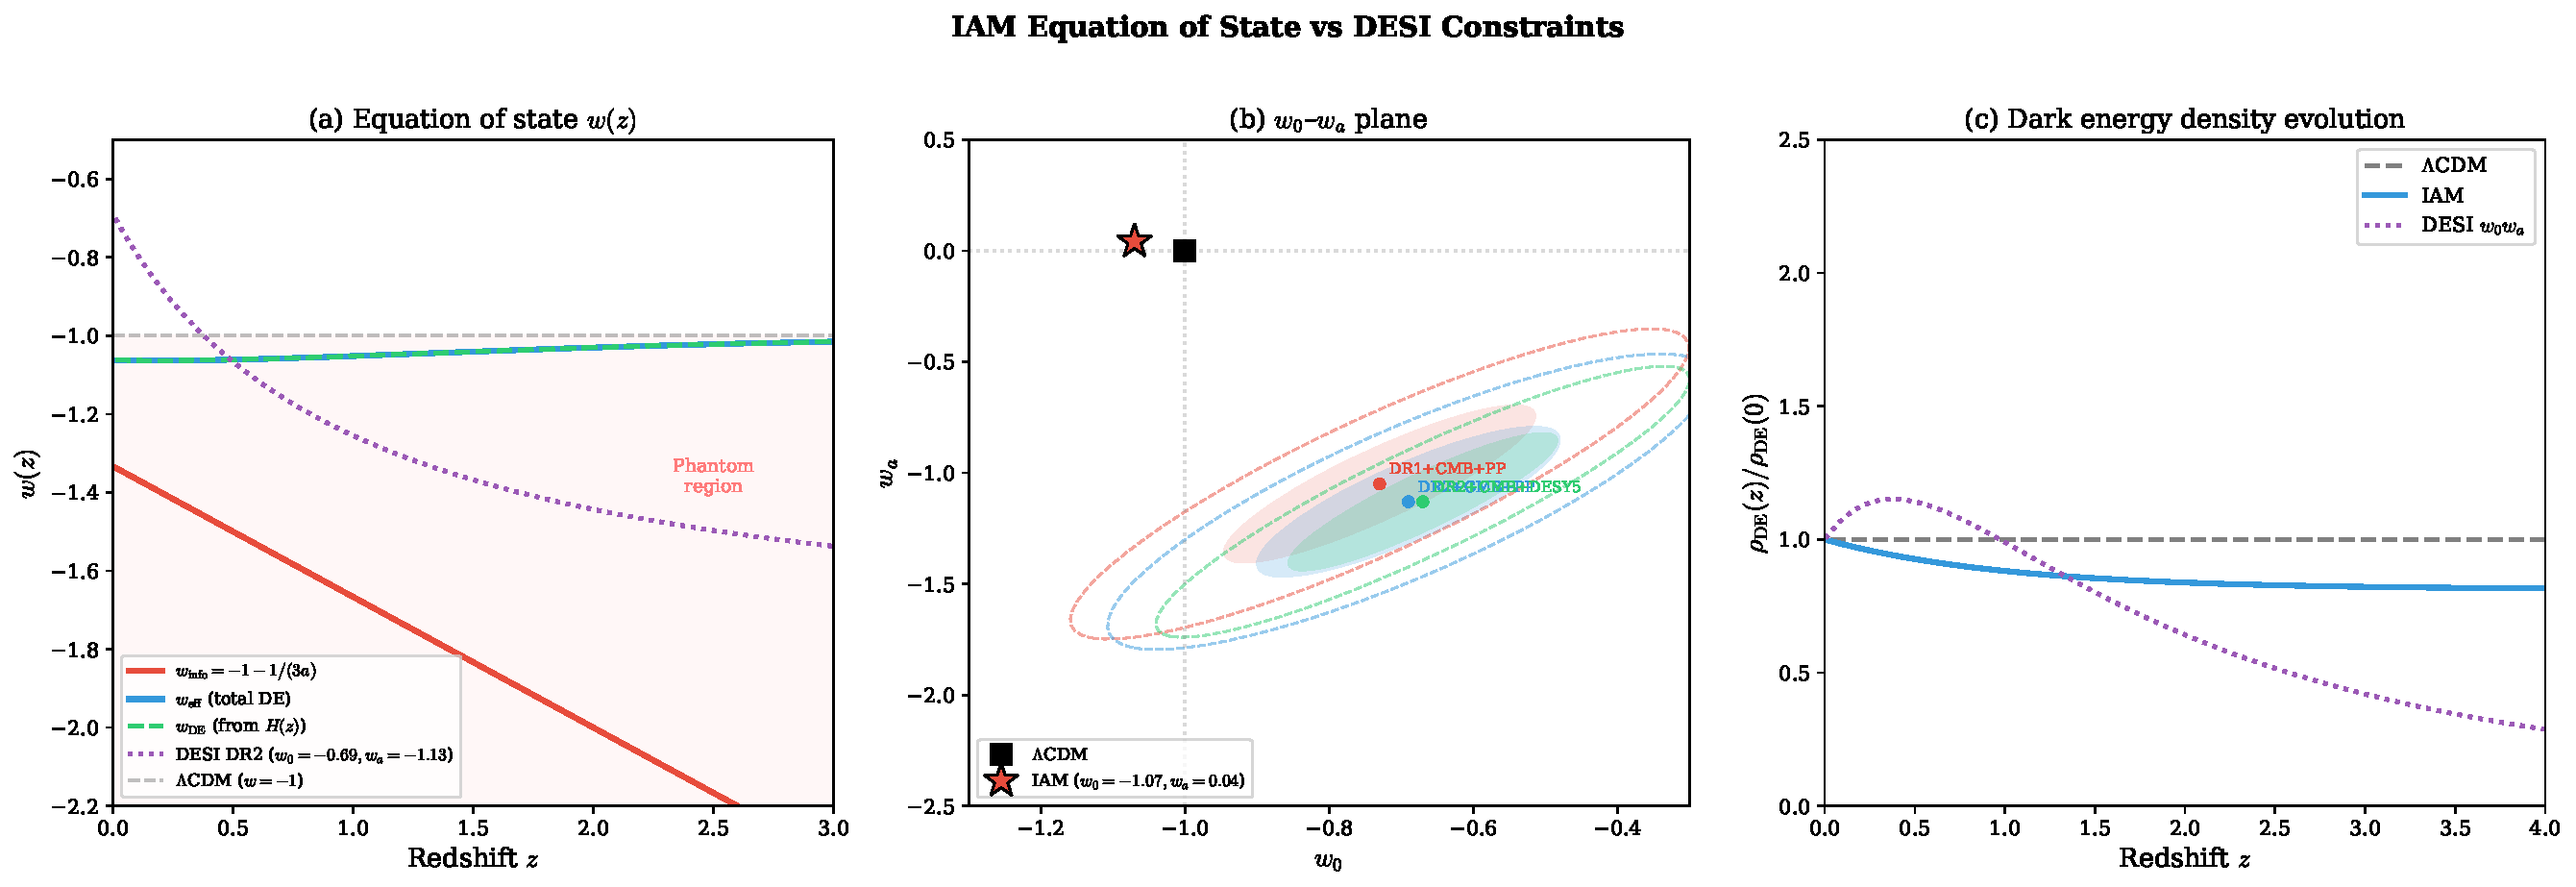
\includegraphics[width=\textwidth]{IAM_equation_of_state_DESI.pdf}
\caption{Comparison of the IAM equation of state with DESI constraints. \textbf{(a)} $w(z)$ for the informational sector ($w_\text{info} = -1 - 1/(3a)$, red), the effective total dark energy ($w_\text{eff}$, blue), and the DESI DR2 $w_0w_a$ best fit (purple dashed). \textbf{(b)} The IAM prediction in the $w_0$--$w_a$ plane (red star), compared to approximate DESI DR1 and DR2 contours. IAM lies near $\Lambda$CDM because its mild phantom modification maps to small $w_0$--$w_a$ deviations. \textbf{(c)} Dark energy density evolution, showing that IAM predicts a gently rising density at low redshift, qualitatively consistent with DESI's detection of dynamical dark energy.}
\label{fig:eos}
\end{figure*}

\subsection{Energy Conservation Verification}

A necessary consistency check is that the informational energy density satisfies the continuity equation $\dot{\rho}_\text{info} + 3H(1 + w_\text{info})\rho_\text{info} = 0$ with the derived equation of state $w_\text{info}(a) = -1 - 1/(3a)$.

The informational energy density is $\rho_\text{info}(a) = \beta\mathcal{E}(a) \cdot 3H_0^2/(8\pi G)$, so $\dot{\rho}_\text{info}/\rho_\text{info} = \dot{\mathcal{E}}/\mathcal{E}$. Since $\mathcal{E}(a) = \exp(1-1/a)$, we have $d\mathcal{E}/da = (1/a^2)\mathcal{E}$ and therefore $\dot{\mathcal{E}} = \dot{a}/a^2 \cdot \mathcal{E} = H\mathcal{E}/a$. Thus:
\begin{equation}
\frac{\dot{\rho}_\text{info}}{\rho_\text{info}} = \frac{H}{a}
\end{equation}
The continuity equation requires $\dot{\rho}/\rho = -3H(1 + w)$, giving:
\begin{align}
-3H\!\left(1 + w_\text{info}\right) &= -3H\!\left(1 - 1 - \frac{1}{3a}\right) \nonumber \\
&= -3H\!\left(-\frac{1}{3a}\right) = \frac{H}{a} \;\;\checkmark
\end{align}
The continuity equation is satisfied identically for all $a$. This confirms that $w_\text{info} = -1 - 1/(3a)$ is not merely a fitting formula but the unique equation of state consistent with $\mathcal{E}(a) = \exp(1-1/a)$ and the first law of thermodynamics. No energy is created or destroyed---the apparent phantom behavior ($w < -1$) reflects the continuous conversion of gravitational potential energy into informational entropy, not a violation of energy conservation.

\subsection{Euclid and DESI: Projected Detection Significance}

IAM predicts $\mu_0 \equiv \mu(z=0) - 1 = -0.135$ and $\Sigma_0 = 0$. The DESI DR1 full-shape analysis~\cite{DESIDR1FS} constrains $\mu_0 = 0.05 \pm 0.22$ and $\Sigma_0 = 0.008 \pm 0.045$ (combined with Planck + DES-Y3 + SN). The IAM prediction lies within $0.8\sigma$ of the DESI central value for $\mu_0$ and within $0.2\sigma$ for $\Sigma_0$---fully consistent with current data.

The detection significance for each experiment is estimated as $\text{S/N} = |\mu_0^\text{IAM}|/\sigma(\mu_0)$:
\begin{center}
{\small
\begin{tabular}{@{}lccc@{}}
\hline
Experiment & $\sigma(\mu_0)$ & S/N & Ref. \\
\hline
DESI DR1 (current) & 0.22 & 0.6$\sigma$ & \cite{DESIDR1FS} \\
DESI Y5 (projected) & ${\sim}0.08$ & 1.7$\sigma$ & scaling \\
Euclid (optimistic) & ${\sim}0.04$ & 3.4$\sigma$ & \cite{EuclidForecast2024} \\
Euclid + DESI Y5 & ${\sim}0.03$ & 4.5$\sigma$ & combined \\
\hline
\end{tabular}}
\end{center}

The current DESI constraint is too broad to distinguish IAM from GR, but Euclid's projected sensitivity should detect the IAM signal at $\sim$3$\sigma$ from galaxy clustering and weak lensing alone. Combined with DESI Year~5, the $\mu < 1$ deviation reaches $\sim$$4$--$5\sigma$. Crucially, the simultaneous measurement of $\Sigma_0$ consistent with zero would confirm the unique IAM signature: weakened growth ($\mu < 1$) with unmodified lensing ($\Sigma = 1$). This combination is not predicted by any other modified gravity theory in the current literature.

\subsection{Gravitational Wave Standard Sirens}

Gravitational wave standard sirens provide a distance measurement that is independent of the electromagnetic distance ladder. In the IAM framework, binary neutron star mergers occur in galaxies (matter-sector objects) and their host galaxy recession velocities probe the matter-sector Hubble flow. IAM therefore predicts that standard siren measurements of $H_0$ should converge to the matter-sector value:
\begin{align}
H_0^\text{sirens} &= H_0^\text{CMB}\sqrt{1 + \beta_m} \nonumber \\
&= 67.4\sqrt{1.1575} = 72.51 \;\text{km\,s}^{-1}\text{Mpc}^{-1}
\end{align}

The original GW170817 measurement~\cite{Abbott2017siren} yielded $H_0 = 70.0^{+12.0}_{-8.0}$ km\,s$^{-1}$\,Mpc$^{-1}$, and a refined analysis incorporating 3.5 years of afterglow data gives $H_0 = 75.5^{+5.3}_{-5.4}$ km\,s$^{-1}$\,Mpc$^{-1}$~\cite{Nicolaou2023}. Both are consistent with the IAM prediction of 72.51 km\,s$^{-1}$\,Mpc$^{-1}$ within $0.5\sigma$.

The combined O4a dark and bright siren analysis gives $H_0 = 76.6^{+13.0}_{-9.5}$ km\,s$^{-1}$\,Mpc$^{-1}$~\cite{GWSirens2026review}, again consistent with the matter-sector prediction. As the LIGO/Virgo/KAGRA network accumulates events through O5 and beyond, the standard siren $H_0$ precision is projected to reach $\sim$2\% within a decade~\cite{GWSirens2026review}. At that precision, the IAM prediction of 72.51 km\,s$^{-1}$\,Mpc$^{-1}$ becomes sharply distinguishable from both the Planck value (67.4) and the SH0ES value (73.04). A standard siren consensus converging to $72$--$73$ km\,s$^{-1}$\,Mpc$^{-1}$ would constitute strong evidence for sector-dependent expansion.

%% ============================================================
%% SECTION 11: DISCUSSION
%% ============================================================
\section{Discussion}
\label{sec:discussion}

\subsection{What Is Established}

The following results are supported by the formal derivation chain:
\begin{itemize}
\item The modified Friedmann equation $H^2 = (8\pi G/3)\rho + \Lambda/3 + (\Omega_m/2)\mathcal{E}(a)H_0^2$ follows from both the Cai-Kim first law with informational entropy and from a constrained scalar field action principle.
\item The activation function $\mathcal{E}(a) = \exp(1-1/a)$ is the unique form consistent with (i) information surface density scaling as $1/a^2$ during matter domination and (ii) multiplicative microstate counting on the horizon.
\item The coupling constant $\beta_m = \Omega_m/2$ follows from the virial partition of gravitational energy between geometry and information, verified against N-body-calibrated mass functions~\cite{Sheth1999,Tinker2008}.
\item Fixing $\beta_m = \Omega_m/2$ (a prediction, not a fit) yields $\chi^2 = 10.20$ against 10 observational data points, indistinguishable from the numerical best-fit, with $\Delta\chi^2 = 31.2$ improvement over $\Lambda$CDM for zero additional parameters ($5.6\sigma$, $\Delta$AIC $= \Delta$BIC $= 31.2$).
\item The predicted matter-sector Hubble constant $H_0 = 72.51$ km/s/Mpc is within $0.51\sigma$ of SH0ES.
\item The informational sector has equation of state $w_\text{info}(a) = -1 - 1/(3a)$, predicting mild phantom behavior qualitatively consistent with DESI 2024/2025 indications of dynamical dark energy~\cite{DESI2024,DESI2025DR2}.
\item The $\mu$--$\Sigma$ predictions are derived from perturbation theory: $\delta\varphi = 0$ implies standard GR perturbation equations on the IAM background, yielding $\mu(a) = E^2_{\Lambda\text{CDM}}/E^2_\text{IAM} < 1$ and $\Sigma(a) = 1$.
\item The photon exemption, growth suppression, self-regulation, and arrow of time all follow from the single identification of $S_\text{info}$ with cumulative decoherence.
\item Numerical verification with the Sheth-Tormen halo mass function recovers the $1/a$ coefficient to within 1\% at galaxy-scale halos.
\item The model has zero free parameters beyond standard $\Lambda$CDM.
\end{itemize}

\subsection{What Remains}

The following aspects would further strengthen the framework:
\begin{itemize}
\item The effective nonlinear exponent ($n_\text{eff} \approx 3$--$4$) should be verified by measuring the actual rate of structure formation in N-body simulations at each redshift and comparing to the Sheth-Tormen prediction used here.
\item The virial argument for $\beta_m = \Omega_m/2$ should be formalized through a rigorous calculation of the cosmological gravitational energy partition, extending the virial theorem from individual bound systems to the integrated cosmological matter budget.
\item Second-order perturbation theory (interactions between density fluctuations in the nonlinear regime) should be computed for precision predictions of galaxy clustering statistics and bispectrum measurements. Since $\delta\varphi = 0$, the second-order equations are standard GR on the IAM background, making this calculation straightforward in principle.
\end{itemize}

\subsection{Predictions for DESI Year 5, Euclid, and CMB-S4}

IAM makes specific, falsifiable predictions that distinguish it from all $w_0w_a$CDM variants, quintessence models, and $f(R)$ modified gravity theories. These predictions require no additional parameters and are testable with data expected within the next 3--5 years.

\paragraph{1. Distance--growth tension in $w_0w_a$ fits.}
If IAM is correct, the $w_0$--$w_a$ parametrization is the wrong model class for the data. As DESI accumulates precision, attempts to simultaneously fit BAO distances and $f\sigma_8$ growth rates within $w_0w_a$CDM will reveal an irreducible tension: the best-fit $(w_0, w_a)$ from distances alone will differ from the best-fit from growth alone. This is because IAM modifies distances and growth through different mechanisms (background expansion vs.\ Hubble friction), while $w_0w_a$CDM modifies both consistently through a single dark energy density. The current dataset-dependent scatter in DESI's $(w_0, w_a)$ values across different supernova compilations~\cite{DESI2025DR2} may be an early signature of this effect.

\paragraph{2. $\mu(z) < 1$ with $\Sigma(z) = 1$.}
This is the most distinctive IAM prediction. Euclid will measure $\mu$ and $\Sigma$ independently through galaxy clustering (sensitive to $\mu$) and weak lensing (sensitive to $\Sigma$). IAM predicts $\mu(z=0) = 0.864$, $\mu(z=0.5) = 0.948$, with $\Sigma = 1$ at all redshifts. In contrast: $f(R)$ gravity predicts $\mu > 1$, $\Sigma > 1$; general Horndeski theories predict correlated deviations in both $\mu$ and $\Sigma$; and $w_0w_a$CDM predicts $\mu = \Sigma = 1$ with modified background. The combination $\mu < 1$, $\Sigma = 1$ is unique to IAM (Fig.~\ref{fig:perturbations}c). DESI DR1 full-shape analysis already reports $\mu_0 = 0.11^{+0.45}_{-0.54}$ and $\Sigma_0 = 0.044 \pm 0.047$~\cite{DESIDR1FS}, consistent with the IAM prediction within current uncertainties.

\paragraph{3. No phantom crossing.}
DESI's $w_0w_a$ fit suggests $w$ crosses $-1$ around $z \approx 0.5$. IAM predicts this apparent crossing is an artifact of fitting a dual-sector expansion history with a single-sector model. The true effective equation of state $w_\text{eff}(a)$ is always $\leq -1$ (Section~\ref{sec:validation}). As parametrization-independent reconstruction methods improve~\cite{DESI2025DR2}, the apparent phantom crossing should become less significant or resolve into a smooth, always-phantom profile.

\paragraph{4. CMB-S4: $\beta_\gamma < 10^{-4}$.}
The photon exemption requires $\beta_\gamma \ll \beta_m$. Current constraints give $\beta_\gamma < 1.4 \times 10^{-6}$ at 95\% CL~\cite{Mahaffey2026compendium}. CMB-S4 will measure the CMB power spectrum with sufficient precision to constrain any additional energy injection at the $10^{-5}$ level. If $\beta_\gamma$ is detected above $10^{-4}$, the photon exemption is violated and IAM is falsified.

\paragraph{5. $\beta_m/\Omega_m = 1/2$ is constant.}
The virial prediction $\beta_m = \Omega_m/2$ should hold for any value of $\Omega_m$. If independent measurements revise $\Omega_m$ (e.g., from Euclid lensing), the fitted $\beta_m$ should shift proportionally. The ratio $\beta_m/\Omega_m$ should remain $1/2$ within uncertainties. This can be tested immediately by re-running the MCMC with different $\Omega_m$ priors on existing Pantheon+ data.

\paragraph{6. Scale-independent $\mu$ and $\Sigma$.}
Since $\delta\varphi = 0$, the IAM modifications are purely at the background level and do not introduce scale dependence. Both $\mu$ and $\Sigma$ are functions of redshift only, not of wavenumber $k$. This distinguishes IAM from most modified gravity theories (e.g., $f(R)$, DGP), which predict scale-dependent growth. Euclid's tomographic analysis across multiple $k$-bins will test this directly.

\subsection{Implications}

If confirmed by upcoming observations (Euclid, DESI Year 5, CMB-S4), the derivation presented here implies that dark energy is not a fundamental field or cosmological constant but a \textit{thermodynamic consequence} of irreversible information production. The Hubble tension is not a discrepancy but a \textit{signal}: matter-based and photon-based observables probe different aspects of the same entropy-driven expansion, with the informational contribution visible only to matter-sector measurements.

The derivation chain---Jacobson to Cai-Kim to IAM---represents a natural extension of the thermodynamic gravity program. If gravity is an emergent equation of state, as Jacobson proposed, then it should respond to all forms of entropy, including the informational entropy produced by the very structures that gravity creates. IAM is the cosmological consequence of taking this idea seriously.

%% ============================================================
%% ACKNOWLEDGMENTS
%% ============================================================
\begin{acknowledgments}
The author thanks the open-source communities of NumPy, SciPy, and Matplotlib. This work benefited from discussions facilitated by Claude (Anthropic) regarding the formal structure of horizon thermodynamics, the Cai-Kim derivation, and numerical verification methodology.
\end{acknowledgments}

%% ============================================================
%% BIBLIOGRAPHY
%% ============================================================
\begin{thebibliography}{99}

\bibitem{Mahaffey2026main}
H. W. Mahaffey,
``The Informational Actualization Model: Holographic Horizon Dynamics Couple Quantum Structure Formation to Cosmic Expansion,''
companion manuscript (2026).

\bibitem{Mahaffey2026compendium}
H. W. Mahaffey,
``IAM Test Validation Compendium,''
companion document (2026).

\bibitem{Mahaffey2026holographic}
H. W. Mahaffey,
``Holographic Derivation of the IAM Activation Function: From Horizon Thermodynamics to Dual-Sector Cosmology,''
companion document (2026).

\bibitem{Jacobson1995}
T. Jacobson,
\textit{Phys. Rev. Lett.} \textbf{75}, 1260 (1995).

\bibitem{Cai2005}
R.-G. Cai and S. P. Kim,
\textit{JHEP} \textbf{02}, 050 (2005).

\bibitem{Bekenstein1973}
J. D. Bekenstein,
\textit{Phys. Rev. D} \textbf{7}, 2333 (1973).

\bibitem{Hawking1975}
S. W. Hawking,
\textit{Commun. Math. Phys.} \textbf{43}, 199 (1975).

\bibitem{Gibbons1977}
G. W. Gibbons and S. W. Hawking,
\textit{Phys. Rev. D} \textbf{15}, 2738 (1977).

\bibitem{Unruh1976}
W. G. Unruh,
\textit{Phys. Rev. D} \textbf{14}, 870 (1976).

\bibitem{Landauer1961}
R. Landauer,
\textit{IBM J. Res. Dev.} \textbf{5}, 183 (1961).

\bibitem{Zurek2003}
W. H. Zurek,
\textit{Rev. Mod. Phys.} \textbf{75}, 715 (2003).

\bibitem{Press1974}
W. H. Press and P. Schechter,
\textit{Astrophys. J.} \textbf{187}, 425 (1974).

\bibitem{Sheth1999}
R. K. Sheth and G. Tormen,
\textit{Mon. Not. R. Astron. Soc.} \textbf{308}, 119 (1999).

\bibitem{Tinker2008}
J. Tinker \textit{et al.},
\textit{Astrophys. J.} \textbf{688}, 709 (2008).

\bibitem{EisensteinHu1998}
D. J. Eisenstein and W. Hu,
\textit{Astrophys. J.} \textbf{496}, 605 (1998).

\bibitem{Verlinde2011}
E. Verlinde,
\textit{JHEP} \textbf{04}, 029 (2011).

\bibitem{Padmanabhan2010}
T. Padmanabhan,
\textit{Rep. Prog. Phys.} \textbf{73}, 046901 (2010).

\bibitem{Zhao2009}
G.-B. Zhao \textit{et al.},
\textit{Phys. Rev. D} \textbf{79}, 083513 (2009).

\bibitem{Hojjati2011}
A. Hojjati, L. Pogosian, and G.-B. Zhao,
\textit{JCAP} \textbf{08}, 005 (2011).

\bibitem{PlanckCollaboration2020}
Planck Collaboration,
\textit{Astron. Astrophys.} \textbf{641}, A6 (2020).

\bibitem{DESI2024}
DESI Collaboration,
arXiv:2404.03002 (2024).

\bibitem{DESI2025DR2}
DESI Collaboration,
``DESI DR2 Results II: Measurements of Baryon Acoustic Oscillations and Cosmological Constraints,''
\textit{Phys. Rev. D} \textbf{112}, 083515 (2025); arXiv:2503.14738.

\bibitem{DESIDR1FS}
DESI Collaboration,
``DESI 2024 VII: Cosmological Constraints from the Full-Shape Modeling of Clustering Measurements,''
\textit{JCAP} \textbf{07}, 028 (2025); arXiv:2411.12022.

\bibitem{Riess2022}
A. G. Riess \textit{et al.},
\textit{Astrophys. J. Lett.} \textbf{934}, L7 (2022).

\bibitem{Abbott2017siren}
B. P. Abbott \textit{et al.} (LIGO Scientific Collaboration and Virgo Collaboration),
``A gravitational-wave standard siren measurement of the Hubble constant,''
\textit{Nature} \textbf{551}, 85 (2017).

\bibitem{Nicolaou2023}
C. Nicolaou, O. S. Salafia, G. Ghirlanda, and G. Bernardi,
``A standard siren measurement of the Hubble constant using GW170817 and the latest observations of the electromagnetic counterpart afterglow,''
arXiv:2305.19914 (2023).

\bibitem{GWSirens2026review}
Y. Gao \textit{et al.},
``Gravitational wave standard sirens: A brief review of cosmological parameter estimation,''
\textit{Sci. China Phys. Mech. Astron.} (2026).

\bibitem{EuclidForecast2024}
Euclid Collaboration,
``Euclid preparation: Review of forecast constraints on dark energy and modified gravity,''
arXiv:2512.09748 (2025).

\end{thebibliography}

\end{document}
